\documentclass[5pt,aspectratio=169]{beamer}
\usetheme{metropolis}
\usepackage{tikz}
\usepackage{amsmath,amssymb,amsthm}
\usepackage{xcolor}
\usepackage{booktabs}
\usepackage{algorithm}
\usepackage{algorithmic}
\usepackage{pgfplots}
\usepackage{attachfile}
\usetikzlibrary{arrows,shapes,positioning,fit,bayesnet,calc,decorations.pathreplacing,backgrounds}




% Theme settings
%\usetheme{Madrid}
%\usecolortheme{whale}
\setbeamertemplate{navigation symbols}{}
%\setbeamertemplate{footline}[frame number]

% Title information
\title{Variational Autoencoders: Theory and Applications}
\author{Mari Ganesh Kumar}
\date{\today}

\AtBeginSection[]{
  \begin{frame}
    \vfill
    \centering
    \begin{beamercolorbox}[sep=8pt,center]{title}
      \usebeamerfont{title}\insertsectionhead\par%
    \end{beamercolorbox}
    \vfill
  \end{frame}
}

\begin{document}

% Title slide
\begin{frame}
  \titlepage
\end{frame}

% Table of contents
\begin{frame}{Outline}
  \tableofcontents
\end{frame}

%%%%%%%%%%%%%%%%%%%%%%%%%%%%%%%%%%%%%%%%%%%%%%%%%%%%%%%%%%%%%%%%%%%%%%%
% Section 3.1: Introduction to Autoencoders & VAEs (30 minutes)
%%%%%%%%%%%%%%%%%%%%%%%%%%%%%%%%%%%%%%%%%%%%%%%%%%%%%%%%%%%%%%%%%%%%%%%
\section{Autoencoders (Continuations) \& Introduction to VAEs}

\begin{frame}{Basic Autoencoder Recap}
  \begin{itemize}
    \item Unsupervised learning model for representation learning
    \item Learns to compress data into lower-dimensional encodings
    \item Reconstructs original data from the compressed representation
    \item Two main components:
      \begin{itemize}
        \item \textbf{Encoder}: $x \mapsto z$ (Input data to latent code)
        \item \textbf{Decoder}: $z \mapsto \hat{x}$ (Latent code to reconstructed data)
      \end{itemize}
  \end{itemize}
  
  \centering
  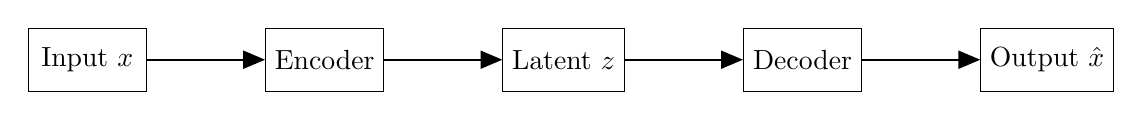
\begin{tikzpicture}[node distance=1.5cm]
    \node[rectangle,draw,minimum width=1.5cm,minimum height=0.8cm] (input) {Input $x$};
    \node[rectangle,draw,minimum width=1.5cm,minimum height=0.8cm,right=of input] (encoder) {Encoder};
    \node[rectangle,draw,minimum width=1.5cm,minimum height=0.8cm,right=of encoder] (latent) {Latent $z$};
    \node[rectangle,draw,minimum width=1.5cm,minimum height=0.8cm,right=of latent] (decoder) {Decoder};
    \node[rectangle,draw,minimum width=1.5cm,minimum height=0.8cm,right=of decoder] (output) {Output $\hat{x}$};
    
    \draw[->,thick] (input) -- (encoder);
    \draw[->,thick] (encoder) -- (latent);
    \draw[->,thick] (latent) -- (decoder);
    \draw[->,thick] (decoder) -- (output);
  \end{tikzpicture}
\end{frame}

\begin{frame}{Deterministic Encoder-Decoder Framework}
  \begin{columns}
    \column{0.6\textwidth}
    \begin{itemize}
      \item Traditional autoencoders use deterministic functions
      \item Encoder: $z = f_{\phi}(x)$
        \begin{itemize}
          \item Maps input $x$ to a fixed point in latent space
          \item Parameterized by weights $\phi$
        \end{itemize}
      \item Decoder: $\hat{x} = g_{\theta}(z)$
        \begin{itemize}
          \item Reconstructs input from latent representation
          \item Parameterized by weights $\theta$
        \end{itemize}
      \item Training objective: minimize reconstruction error
        \begin{align}
          \mathcal{L}(x, \hat{x}) = \|x - g_{\theta}(f_{\phi}(x))\|^2
        \end{align}
    \end{itemize}
    
    \column{0.4\textwidth}
    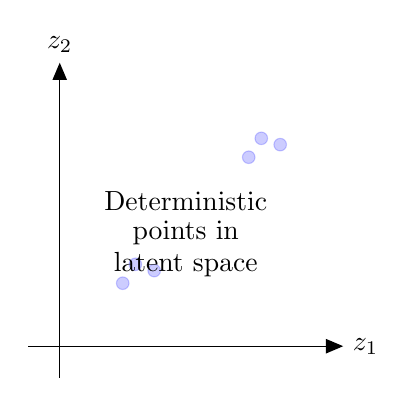
\begin{tikzpicture}[scale=0.8]
      \draw[->] (-0.5,0) -- (4.5,0) node[right] {$z_1$};
      \draw[->] (0,-0.5) -- (0,4.5) node[above] {$z_2$};
      
      \filldraw[blue, opacity=0.2] (1,1) circle (0.1);
      \filldraw[blue, opacity=0.2] (1.2,1.3) circle (0.1);
      \filldraw[blue, opacity=0.2] (1.5,1.2) circle (0.1);
      \filldraw[blue, opacity=0.2] (3,3) circle (0.1);
      \filldraw[blue, opacity=0.2] (3.2,3.3) circle (0.1);
      \filldraw[blue, opacity=0.2] (3.5,3.2) circle (0.1);
      
      \node at (2,2.3) {Deterministic};
      \node at (2,1.8) {points in};
      \node at (2,1.3) {latent space};
    \end{tikzpicture}
  \end{columns}
\end{frame}

\begin{frame}{Bottleneck and Dimensionality Reduction}
  \begin{columns}
    \column{0.55\textwidth}
    \begin{itemize}
      \item Latent space has lower dimensionality than input
      \item Forces network to learn efficient representations
      \item Bottleneck architecture:
        \begin{itemize}
          \item Input: high-dimensional data (e.g., 784D for MNIST)
          \item Latent: low-dimensional (e.g., 2-100D)
          \item Output: same dimension as input
        \end{itemize}
      \item Similar to PCA but can capture non-linear relationships
      \item Training learns to extract most important features
    \end{itemize}
    
    \column{0.45\textwidth}
    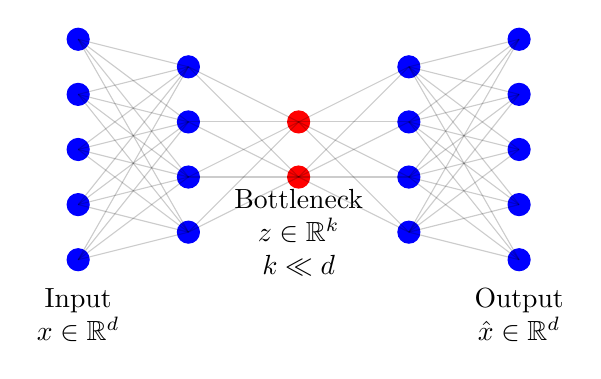
\begin{tikzpicture}[scale=0.7]
      % Input layer
      \foreach \y in {1,...,5}
        \filldraw[blue] (0,\y) circle (0.2);
      
      % Hidden layer 1
      \foreach \y in {1.5,...,4.5}
        \filldraw[blue] (2,\y) circle (0.2);
        
      % Bottleneck layer
      \foreach \y in {2.5,3.5}
        \filldraw[red] (4,\y) circle (0.2);
      
      % Hidden layer 2
      \foreach \y in {1.5,...,4.5}
        \filldraw[blue] (6,\y) circle (0.2);
      
      % Output layer
      \foreach \y in {1,...,5}
        \filldraw[blue] (8,\y) circle (0.2);
      
      % Connections
      \foreach \i in {1,...,5}
        \foreach \j in {1.5,2.5,3.5,4.5}
          \draw[-, opacity=0.2] (0,\i) -- (2,\j);
          
      \foreach \i in {1.5,2.5,3.5,4.5}
        \foreach \j in {2.5,3.5}
          \draw[-, opacity=0.2] (2,\i) -- (4,\j);
          
      \foreach \i in {2.5,3.5}
        \foreach \j in {1.5,2.5,3.5,4.5}
          \draw[-, opacity=0.2] (4,\i) -- (6,\j);
          
      \foreach \i in {1.5,2.5,3.5,4.5}
        \foreach \j in {1,...,5}
          \draw[-, opacity=0.2] (6,\i) -- (8,\j);
      
      % Labels
      \node[align=center] at (0,0) {Input\\$x \in \mathbb{R}^d$};
      \node[align=center] at (4,1.5) {Bottleneck\\$z \in \mathbb{R}^k$\\$k \ll d$};
      \node[align=center] at (8,0) {Output\\$\hat{x} \in \mathbb{R}^d$};
    \end{tikzpicture}
  \end{columns}
\end{frame}

\begin{frame}{Application 1: Data Compression}
  \begin{columns}
    \column{0.7\textwidth}
    \begin{itemize}
      \item \textbf{Scenario}: Storage of massive document images (e.g., Billing Images)
      \item \textbf{Approach}: Compress raw high-dimensional images to a 256-dimensional latent space
      \item \textbf{Storage Savings}: Achieve significant storage reduction
        \begin{itemize}
          \item Raw: $256 \times 256 \times 3 \times 1\text{ Billion} \times 1\text{ byte per pixel}$
          \item Compressed: $256 \times 1\text{ Billion} \times 1\text{ byte per dimension}$
        \end{itemize}
      \item \textbf{Trade-offs}:
        \begin{itemize}
          \item Aggressive savings $\rightarrow$ low quality reconstruction
          \item Better/advanced modelling $\rightarrow$ better reconstruction \& better savings
        \end{itemize}
    \end{itemize}
    
    \column{0.29\textwidth}
    \centering
    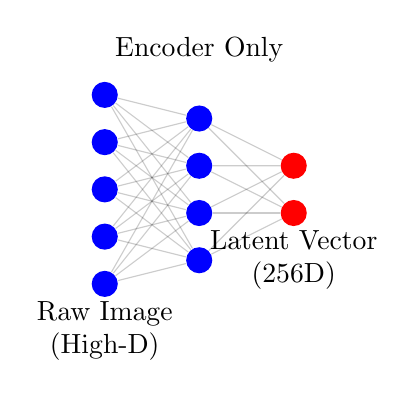
\begin{tikzpicture}[scale=0.6]
      % Input layer
      \foreach \y in {1,...,5}
        \node[circle, fill=blue, minimum size=0.3cm] (i\y) at (0,\y) {};
      
      % Hidden layer 1
      \foreach \y [count=\yi] in {1.5,2.5,3.5,4.5}
        \node[circle, fill=blue, minimum size=0.3cm] (h\yi) at (2,\y) {};
        
      % Bottleneck layer
      \foreach \y [count=\yi] in {2.5,3.5}
        \node[circle, fill=red, minimum size=0.3cm] (b\yi) at (4,\y) {};
      
      % Connections
      \foreach \i in {1,...,5}
        \foreach \j in {1,...,4}
          \draw[-, opacity=0.2] (i\i) -- (h\j);
          
      \foreach \i in {1,...,4}
        \foreach \j in {1,2}
          \draw[-, opacity=0.2] (h\i) -- (b\j);
      
      % Labels
      \node[align=center] at (0,0) {Raw Image\\(High-D)};
      \node[align=center] at (4,1.5) {Latent Vector\\(256D)};
      
      \node[align=center, above] at (2,5.5) {Encoder Only};
    \end{tikzpicture}
  \end{columns}
\end{frame}

\begin{frame}{Application 2: Unsupervised Pre-training}
  \begin{columns}
    \column{0.55\textwidth}
    \begin{itemize}
      \item \textbf{Problem}: Limited labeled data for image classification
      \item \textbf{Scenario}:
        \begin{itemize}
          \item $1,000,000$ photos \textbf{without labels}
          \item $1,000$ photos \textbf{with labels}
        \end{itemize}
      \item \textbf{Approach}:
        \begin{enumerate}
          \item Pre-train the encoder using all 1M unlabeled photos (learn generic features)
          \item Retain the trained Encoder and add a thin classification head
          \item Train the classification head on the 1,000 labeled photos
        \end{enumerate}
    \end{itemize}
    
    \column{0.45\textwidth}
    \centering
    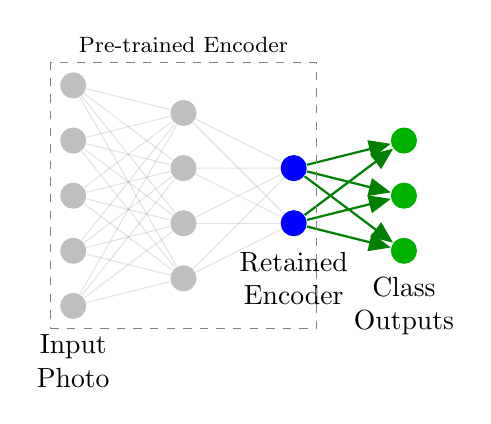
\begin{tikzpicture}[scale=0.7]
      % Input layer
      \foreach \y in {1,...,5}
        \node[circle, fill=gray!50, minimum size=0.3cm] (i\y) at (0,\y) {};
      
      % Hidden layer 1
      \foreach \y [count=\yi] in {1.5,2.5,3.5,4.5}
        \node[circle, fill=gray!50, minimum size=0.3cm] (h\yi) at (2,\y) {};
        
      % Retained Encoder Output
      \foreach \y [count=\yi] in {2.5,3.5}
        \node[circle, fill=blue, minimum size=0.3cm] (b\yi) at (4,\y) {};
        
      % Classification Layer
      \foreach \y [count=\yi] in {2,3,4}
        \node[circle, fill=green!70!black, minimum size=0.3cm] (c\yi) at (6,\y) {};
      
      % Connections (Frozen)
      \foreach \i in {1,...,5}
        \foreach \j in {1,...,4}
          \draw[-, opacity=0.1] (i\i) -- (h\j);
          
      \foreach \i in {1,...,4}
        \foreach \j in {1,2}
          \draw[-, opacity=0.1] (h\i) -- (b\j);
          
      % Connections (Trained)
      \foreach \i in {1,2}
        \foreach \j in {1,2,3}
          \draw[->, thick, green!50!black] (b\i) -- (c\j);
      
      % Labels
      \node[align=center] at (0,0) {Input\\Photo};
      \node[align=center] at (4,1.5) {Retained\\Encoder};
      \node[align=center] at (6,1) {Class\\Outputs};
      
      % Fit box for retained encoder
      \node[draw, dashed, gray, fit=(i1) (i5) (b2), label=above:Pre-trained Encoder] {};
    \end{tikzpicture}
  \end{columns}
\end{frame}

\begin{frame}{Motivation for Probabilistic Modeling}
  \begin{itemize}
    \item Deterministic autoencoders can't:
      \begin{itemize}
        \item Generate new samples effectively
        \item Capture uncertainty in the encoding process
        \item Handle ambiguity in the data
        \item Provide meaningful interpolations
      \end{itemize}
    \item Probabilistic approach:
      \begin{itemize}
        \item Model the encoding as a distribution, not a point
        \item Allow sampling from the latent space
        \item Explicitly capture uncertainty and variability
        \item Enable generative modeling capabilities
      \end{itemize}
    \item Goal: Learn useful probability distributions over the data
  \end{itemize}
  
 
\end{frame}

\begin{frame}

 \centering
  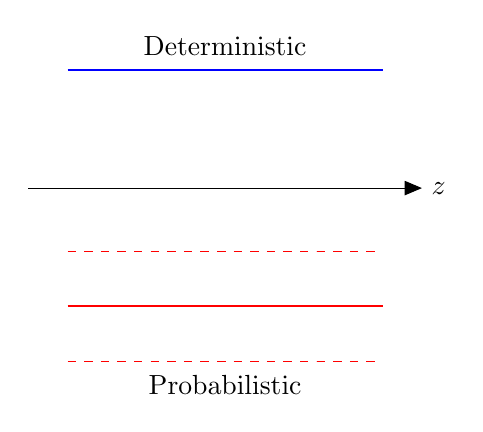
\begin{tikzpicture}
    \draw[->] (0,0) -- (5,0) node[right] {$z$};
    
    % Deterministic mapping
    \draw[domain=0.5:4.5, smooth, variable=\x, blue, thick] plot ({\x}, {1.5});
    \node at (2.5,1.8) {Deterministic};
    
    % Probabilistic mapping
    \draw[domain=0.5:4.5, smooth, variable=\x, red, thick] plot ({\x}, {-1.5});
    \draw[domain=0.5:4.5, smooth, variable=\x, red, dashed] plot ({\x}, {-2.2});
    \draw[domain=0.5:4.5, smooth, variable=\x, red, dashed] plot ({\x}, {-0.8});
    \node at (2.5, -2.5) {Probabilistic};
  \end{tikzpicture}
    
\end{frame}

\begin{frame}{Limitations of Deterministic Embeddings}
  \textbf{Overfitting}
  \begin{itemize}
    \item Deterministic autoencoders often memorize training examples
    \item Poor generalization to unseen data
    \item Can't handle noisy or ambiguous inputs effectively
  \end{itemize}
  
  \textbf{Lack of Generativity}
  \begin{itemize}
    \item No principled way to sample new points from latent space
    \item Random sampling produces unrealistic outputs
    \item No awareness of latent space structure
  \end{itemize}
\end{frame}


\begin{frame}

  \centering
  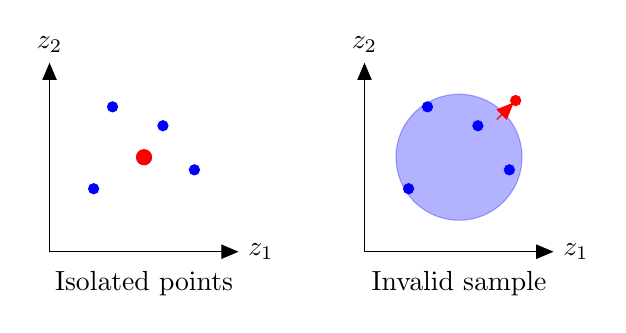
\begin{tikzpicture}[scale=0.8]
    % Left side: deterministic overfitting
    \begin{scope}[shift={(-2.5,0)}]
      \draw[->] (-1.5,-1.5) -- (1.5,-1.5) node[right] {$z_1$};
      \draw[->] (-1.5,-1.5) -- (-1.5,1.5) node[above] {$z_2$};
      
      \filldraw[blue] (-0.8,-0.5) circle (0.08);
      \filldraw[blue] (-0.5,0.8) circle (0.08);
      \filldraw[blue] (0.3,0.5) circle (0.08);
      \filldraw[blue] (0.8,-0.2) circle (0.08);
      \filldraw[red] (0,0) circle (0.12);
      
      \node at (0,-2) {Isolated points};
    \end{scope}
    
    % Right side: sampling issues
    \begin{scope}[shift={(2.5,0)}]
      \draw[->] (-1.5,-1.5) -- (1.5,-1.5) node[right] {$z_1$};
      \draw[->] (-1.5,-1.5) -- (-1.5,1.5) node[above] {$z_2$};
      
      \filldraw[blue, opacity=0.3] (0,0) circle (1);
      \filldraw[blue] (-0.8,-0.5) circle (0.08);
      \filldraw[blue] (-0.5,0.8) circle (0.08);
      \filldraw[blue] (0.3,0.5) circle (0.08);
      \filldraw[blue] (0.8,-0.2) circle (0.08);
      \filldraw[red] (0.9,0.9) circle (0.08);
      \draw[red,->] (0.6,0.6) -- (0.87,0.87);
      
      \node at (0,-2) {Invalid sample};
    \end{scope}
  \end{tikzpicture}
    
\end{frame}



\begin{frame}{Latent Variable Models in Unsupervised Learning}
\begin{columns}
    \column{0.6\textwidth}
     \begin{itemize}
    \item Latent variable: hidden factor that explains observed data
    \item Model structure: $p(x,z) = p(z)p(x|z)$
      \begin{itemize}
        \item $p(z)$: prior distribution over latent variables
        \item $p(x|z)$: likelihood of data given latent variables
      \end{itemize}
    \item Generative process:
      \begin{itemize}
        \item Sample $z \sim p(z)$
        \item Generate $x \sim p(x|z)$
      \end{itemize}
    \item Inference problem: determine $p(z|x)$
    \item Examples of latent variable models:
      \begin{itemize}
        \item Gaussian Mixture Models (GMM)
        \item Hidden Markov Models (HMM)
        \item Variational Autoencoders (VAE)
      \end{itemize}
  \end{itemize}
    \column{0.4\textwidth}
  
  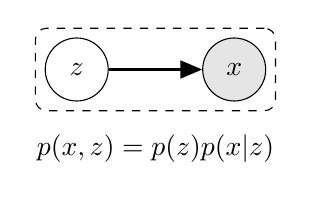
\begin{tikzpicture}
% Graphical model
\node[circle,draw,minimum size=0.8cm] (z) at (0,0) {$z$};
\node[circle,draw,fill=gray!20,minimum size=0.8cm] (x) at (2,0) {$x$};
\draw[->,thick] (z) -- (x);
\node[draw,dashed,fit=(z)(x),rounded corners] {};
\node at (1,-1) {$p(x,z) = p(z)p(x|z)$};
  \end{tikzpicture}
    
\end{columns}
\end{frame}
 



\begin{frame}{Variational Autoencoder (VAE) Fundamentals}
    \begin{itemize}
      \item Combines:
        \begin{itemize}
          \item Autoencoder architecture
          \item Probabilistic latent variable modeling
          \item Variational inference
        \end{itemize}
      \item Key differences from standard autoencoder:
        \begin{itemize}
          \item Encodes to distribution, not point
          \item Uses stochastic sampling in latent space
          \item Includes regularization via KL divergence
          \item Can generate new samples
        \end{itemize}
      \item Framework:
        \begin{itemize}
          \item Encoder: $q_\phi(z|x)$ (approximate posterior)
          \item Decoder: $p_\theta(x|z)$ (likelihood model)
        \end{itemize}
    \end{itemize}
    
    

\end{frame}

\begin{frame}
    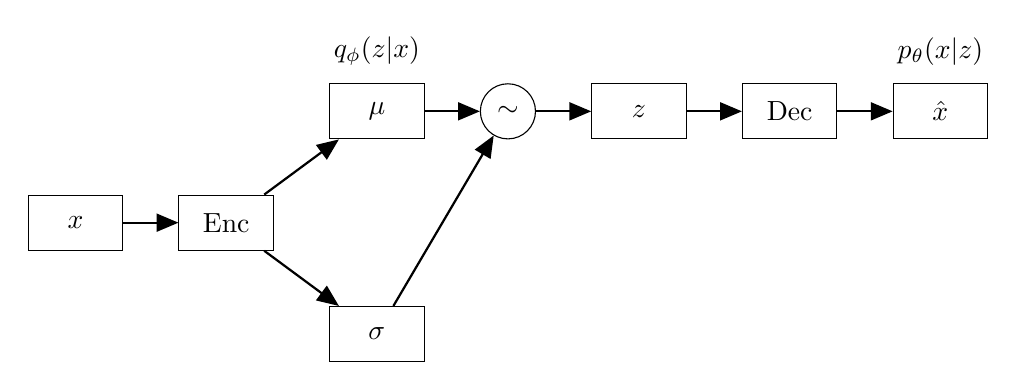
\begin{tikzpicture}[node distance=1.2cm]
      \node[rectangle,draw,minimum width=1.2cm,minimum height=0.7cm] (input) {$x$};
      \node[rectangle,draw,minimum width=1.2cm,minimum height=0.7cm, right=0.7cm of input] (enc) {Enc};
      \node[rectangle,draw,minimum width=1.2cm,minimum height=0.7cm,above right=0.7cm and 0.7cm of enc] (mu) {$\mu$};
      \node[rectangle,draw,minimum width=1.2cm,minimum height=0.7cm,below right=0.7cm and 0.7cm of enc] (sigma) {$\sigma$};
      \node[circle,draw,minimum width=0.7cm,right=0.7cm of mu] (sample) {$\sim$};
      \node[rectangle,draw,minimum width=1.2cm,minimum height=0.7cm,right=0.7cm of sample] (z) {$z$};
      \node[rectangle,draw,minimum width=1.2cm,minimum height=0.7cm,right=0.7cm of z] (decoder) {Dec};
      \node[rectangle,draw,minimum width=1.2cm,minimum height=0.7cm,right=0.7cm of decoder] (output) {$\hat{x}$};
      
      
      \draw[->,thick] (input) -- (enc);
      \draw[->,thick] (enc) -- (mu);
      \draw[->,thick] (enc) -- (sigma);
      \draw[->,thick] (mu) -- (sample);
      \draw[->,thick] (sigma) -- (sample);
      \draw[->,thick] (sample) -- (z);
      \draw[->,thick] (z) -- (decoder);
      \draw[->,thick] (decoder) -- (output);
      
      \node[above=0.1cm of mu] {$q_\phi(z|x)$};
      \node[above=0.1cm of output] {$p_\theta(x|z)$};
    \end{tikzpicture}

\begin{itemize}
\item \textbf{Key innovation}: Combining variational inference with neural networks
\item \textbf{Probabilistic encoder}: Maps inputs to distributions over latent space
\item \textbf{Probabilistic decoder}: Generates data given latent variables
\item \textbf{Training objective}: Evidence Lower Bound (ELBO)
\end{itemize}
    
\end{frame}



\begin{frame}{Encoding to a Distribution Rather Than a Point}
  \begin{columns}
    \column{0.55\textwidth}
    \begin{itemize}
      \item Standard autoencoder:
        \begin{itemize}
          \item $z = f_\phi(x)$ (deterministic)
          \item Each input maps to exactly one point
        \end{itemize}
      \item VAE encoder:
        \begin{itemize}
          \item $q_\phi(z|x) = \mathcal{N}(z; \mu_\phi(x), \sigma^2_\phi(x))$
          \item Each input maps to a distribution
          \item Neural network outputs $\mu_\phi(x)$ and $\log \sigma^2_\phi(x)$
        \end{itemize}
      \item Advantages:
        \begin{itemize}
          \item Captures uncertainty in encoding
          \item Encourages smooth latent space
          \item Enables generative capabilities
          \item More robust to noise
        \end{itemize}
    \end{itemize}
    
    \column{0.45\textwidth}
    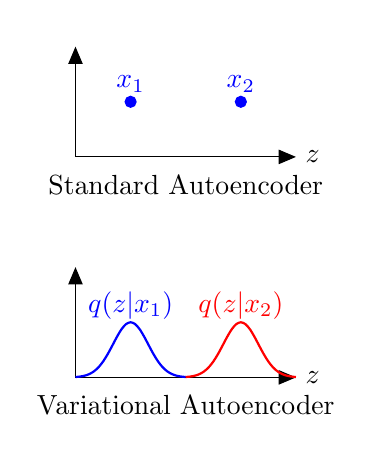
\begin{tikzpicture}[scale=0.7]
      % Standard autoencoder
      \begin{scope}[shift={(0,2)}]
        \draw[->] (0,0) -- (4,0) node[right] {$z$};
        \draw[->] (0,0) -- (0,2) node[above] {};
        \filldraw[blue] (1,1) circle (0.1) node[above] {$x_1$};
        \filldraw[blue] (3,1) circle (0.1) node[above] {$x_2$};
        \node at (2,-0.5) {Standard Autoencoder};
      \end{scope}
      
      % VAE
      \begin{scope}[shift={(0,-2)}]
        \draw[->] (0,0) -- (4,0) node[right] {$z$};
        \draw[->] (0,0) -- (0,2) node[above] {};
        
        % Gaussian for x1
        \draw[domain=0:2, smooth, variable=\x, blue, thick] plot ({\x}, {exp(-(\x-1)^2/0.2)});
        \node[blue] at (1,1.3) {$q(z|x_1)$};
        
        % Gaussian for x2
        \draw[domain=2:4, smooth, variable=\x, red, thick] plot ({\x}, {exp(-(\x-3)^2/0.2)});
        \node[red] at (3,1.3) {$q(z|x_2)$};
        
        \node at (2,-0.5) {Variational Autoencoder};
      \end{scope}
    \end{tikzpicture}
  \end{columns}
\end{frame}




\begin{frame}{Decoder as a Generative Model}
  \begin{columns}
    \column{0.55\textwidth}
    \begin{itemize}
      \item Standard autoencoder decoder:
        \begin{itemize}
          \item Deterministic: $\hat{x} = g_\theta(z)$
          \item Just tries to reconstruct input
        \end{itemize}
      \item VAE decoder:
        \begin{itemize}
          \item Generative model: $p_\theta(x|z)$
          \item Mostly Gaussian (continuous data)
          \item For images: $p_\theta(x|z) = \mathcal{N}(x; g_\theta(z), \sigma^2 I)$
        \end{itemize}
      \item Generative process:
        \begin{itemize}
          \item Sample $z \sim p(z) = \mathcal{N}(0, I)$
          \item Generate $x \sim p_\theta(x|z)$
        \end{itemize}
    \end{itemize}
    
    \column{0.45\textwidth}
    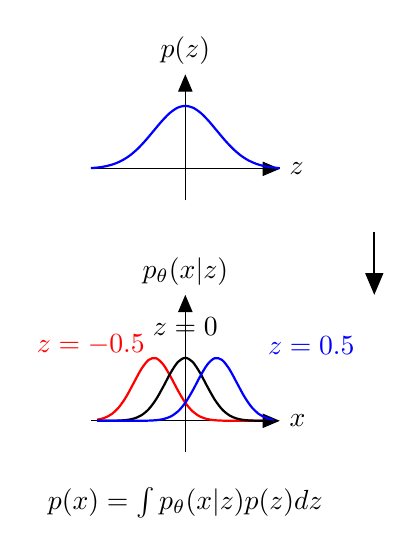
\begin{tikzpicture}[scale=0.8]
      % Prior
      \begin{scope}[shift={(0,3)}]
        \draw[->] (-1.5,0) -- (1.5,0) node[right] {$z$};
        \draw[->] (0,-0.5) -- (0,1.5) node[above] {$p(z)$};
        \draw[domain=-1.5:1.5, smooth, variable=\x, blue, thick] 
          plot ({\x}, {exp(-\x*\x/0.5)});
      \end{scope}
      
      % Arrow down
      \draw[->, thick] (3,2) -- (3,1);
      
      % Conditional
      \begin{scope}[shift={(0,-1)}]
        \draw[->] (-1.5,0) -- (1.5,0) node[right] {$x$};
        \draw[->] (0,-0.5) -- (0, 2) node[above] {$p_\theta(x|z)$};
        
        \draw[domain=-1.4:1.4, smooth, variable=\x, red, thick] 
          plot ({\x}, {exp(-(\x+0.5)^2/0.2)});
        \node[red] at (-1.5,1.2) {$z=-0.5$};
        
        \draw[domain=-1.4:1.4, smooth, variable=\x, black, thick] 
          plot ({\x}, {exp(-(\x)^2/0.2)});
        \node[black] at (0,1.5) {$z=0$};
        
        \draw[domain=-1.4:1.4, smooth, variable=\x, blue, thick] 
          plot ({\x}, {exp(-(\x-0.5)^2/0.2)});
        \node[blue] at (2,1.2) {$z=0.5$};
      \end{scope}
      
      \node at (0,-2.3) {$p(x) = \int p_\theta(x|z)p(z)dz$};
    \end{tikzpicture}
  \end{columns}
\end{frame}



\begin{frame}{VAE vs. Standard Autoencoder}
  \begin{center}
    \begin{tabular}{p{6cm}|p{6cm}}
      \toprule
      \textbf{Standard Autoencoder} & \textbf{Variational Autoencoder} \\
      \midrule
      Deterministic mapping $z = f_\phi(x)$ & Probabilistic mapping $q_\phi(z|x)$ \\
      \midrule
      Point encoding in latent space & Distribution encoding in latent space \\
      \midrule
      Minimizes reconstruction error & Maximizes ELBO (reconstruction + KL) \\
      \midrule
      No regularization of latent space & KL divergence regularizes latent space \\
      \midrule
      Can't generate new samples & Can generate new samples \\
      \midrule
      Discontinuous latent space & Continuous latent space \\
      \midrule
      No probabilistic interpretation & Bayesian probabilistic model \\
      \bottomrule
    \end{tabular}
  \end{center}
  
 
\end{frame}


\begin{frame}
\centering
 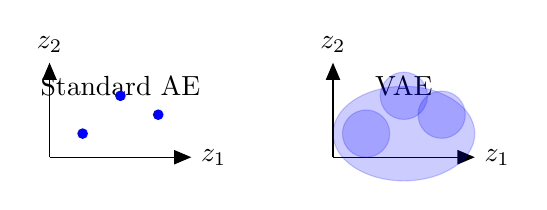
\begin{tikzpicture}[scale=0.6]
    \begin{scope}[shift={(-3,0)}]
      \node at (0,1) {Standard AE};
      \draw[->] (-1.5,-0.5) -- (1.5,-0.5) node[right] {$z_1$};
      \draw[->] (-1.5,-0.5) -- (-1.5,1.5) node[above] {$z_2$};
      \filldraw[blue] (-0.8,0) circle (0.1);
      \filldraw[blue] (0,0.8) circle (0.1);
      \filldraw[blue] (0.8,0.4) circle (0.1);
    \end{scope}
    
    \begin{scope}[shift={(3,0)}]
      \node at (0,1) {VAE};
      \draw[->] (-1.5,-0.5) -- (1.5,-0.5) node[right] {$z_1$};
      \draw[->] (-1.5,-0.5) -- (-1.5,1.5) node[above] {$z_2$};
      \filldraw[blue, opacity=0.2] (-0.8,0) circle (0.5);
      \filldraw[blue, opacity=0.2] (0,0.8) circle (0.5);
      \filldraw[blue, opacity=0.2] (0.8,0.4) circle (0.5);
      \filldraw[blue, opacity=0.2] (0,0) ellipse (1.5 and 1);
    \end{scope}
  \end{tikzpicture}  
  
\end{frame}







\begin{frame}{Applications Overview}
  \textbf{Data Generation}
  \begin{itemize}
    \item Generate new realistic samples
    \item Image synthesis, music generation, text creation
    \item Controlled generation via latent space manipulation
  \end{itemize}
  
  \textbf{Anomaly Detection \& Denosing}
 
  \textbf{Representation Learning}
  \begin{itemize}
    \item Extract meaningful features from unlabeled data
    \item Transfer learning and downstream tasks
    \item Semi-supervised learning applications
  \end{itemize}
\end{frame}

%%%%%%%%%%%%%%%%%%%%%%%%%%%%%%%%%%%%%%%%%%%%%%%%%%%%%%%%%%%%%%%%%%%%%%%
% Section 3.2: Detailed Exploration of VAEs (60 minutes)
%%%%%%%%%%%%%%%%%%%%%%%%%%%%%%%%%%%%%%%%%%%%%%%%%%%%%%%%%%%%%%%%%%%%%%%
\section{Detailed Exploration of VAEs}

\begin{frame}{Detailed Exploration of VAEs}
\begin{itemize}
\item Probabilistic latent variable model framework
\item Generative process and prior distributions
\item Encoder network: inferring latent variables
\item Reparameterization trick for training
\item Decoder network: generating data
\item Sampling and interpolation techniques
\item Implementation considerations
\end{itemize}

\begin{center}
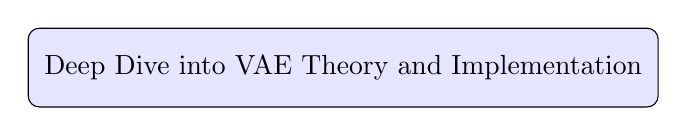
\begin{tikzpicture}
\node[rectangle,draw,fill=blue!10,rounded corners,minimum width=8cm,minimum height=1cm] at (0,0) {Deep Dive into VAE Theory and Implementation};
\end{tikzpicture}
\end{center}
\end{frame}


\begin{frame}{Probabilistic Latent Variable Model}
\begin{itemize}
\item VAE is a latent variable model: $p(x,z) = p(z)p(x|z)$ \textcolor{blue}{($z$ is fixed, $x$ is unknown)}
\item Goal: Maximize likelihood of observed data $p(x)$
\item Problem: $p(x) = \int p(z)p(x|z)dz$ is intractable
\item Solution: Variational approximation with $q(z|x)$ (approximate postierior for $p(z|x)$)
\end{itemize}

\begin{center}
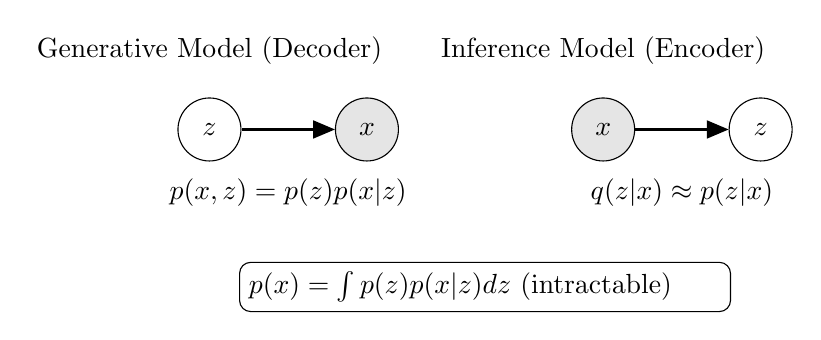
\begin{tikzpicture}
% Generative model
\node at (0,1) {Generative Model (Decoder)};
\node[circle,draw,minimum size=0.8cm] (z1) at (0,0) {$z$};
\node[circle,draw,fill=gray!20,minimum size=0.8cm] (x1) at (2,0) {$x$};
\draw[->,thick] (z1) -- (x1);
\node[below] at (1,-0.5) {$p(x,z) = p(z)p(x|z)$};

% Inference model
\node at (5,1) {Inference Model (Encoder)};
\node[circle,draw,minimum size=0.8cm] (z2) at (7,0) {$z$};
\node[circle,draw,fill=gray!20,minimum size=0.8cm] (x2) at (5,0) {$x$};
\draw[->,thick] (x2) -- (z2);
\node[below] at (6,-0.5) {$q(z|x) \approx p(z|x)$};

% Integration
\node[draw,rounded corners,text width=6cm] at (3.5,-2) {$p(x) = \int p(z)p(x|z)dz$ (intractable)};
\end{tikzpicture}
\end{center}
\end{frame}








\begin{frame}{Encoder Network - Overview}
\begin{itemize}
\item Encoder implements variational approximation $q(z|x)$
\item Amortized inference: single network for all $x$
\item Maps inputs to parameters of $q(z|x)$
\item Design depends on data type (MLP, CNN, RNN, etc.)
\end{itemize}

\begin{center}
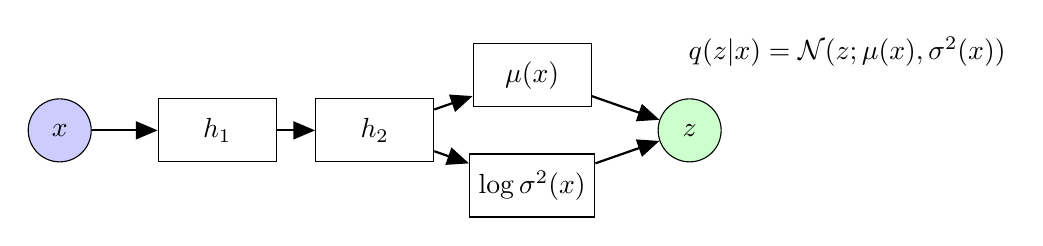
\begin{tikzpicture}
% Encoder network
\node[circle,draw,fill=blue!20,minimum size=0.8cm] (x) at (0,0) {$x$};
\node[rectangle,draw,minimum width=1.5cm,minimum height=0.8cm] (h1) at (2,0) {$h_1$};
\node[rectangle,draw,minimum width=1.5cm,minimum height=0.8cm] (h2) at (4,0) {$h_2$};
\node[rectangle,draw,minimum width=1.5cm,minimum height=0.8cm] (mu) at (6,0.7) {$\mu(x)$};
\node[rectangle,draw,minimum width=1.5cm,minimum height=0.8cm] (logvar) at (6,-0.7) {$\log\sigma^2(x)$};
\node[circle,draw,fill=green!20,minimum size=0.8cm] (z) at (8,0) {$z$};

\draw[->,thick] (x) -- (h1);
\draw[->,thick] (h1) -- (h2);
\draw[->,thick] (h2) -- (mu);
\draw[->,thick] (h2) -- (logvar);
\draw[->,thick] (mu) -- (z);
\draw[->,thick] (logvar) -- (z);

\node at (10,1) {$q(z|x) = \mathcal{N}(z; \mu(x), \sigma^2(x))$};
\end{tikzpicture}
\end{center}
\end{frame}


\begin{frame}{Parameterizing $q(z|x)$ as Gaussian}
  \begin{columns}
    \column{0.5\textwidth}
    \begin{itemize}
      \item We model $q_\phi(z|x)$ as a multivariate Gaussian:
        \begin{align}
          q_\phi(z|x) = \mathcal{N}(z; \mu_\phi(x), \text{diag}(\sigma^2_\phi(x)))
        \end{align}
      
      \item Reasons for Gaussian choice:
        \begin{itemize}
          \item Differentiable sampling (reparameterization)
          \item KL divergence with Gaussian prior has analytic form
          \item Flexible enough for many applications
          \item Computational efficiency
        \end{itemize}
      
    \end{itemize}
    
    \column{0.5\textwidth}
    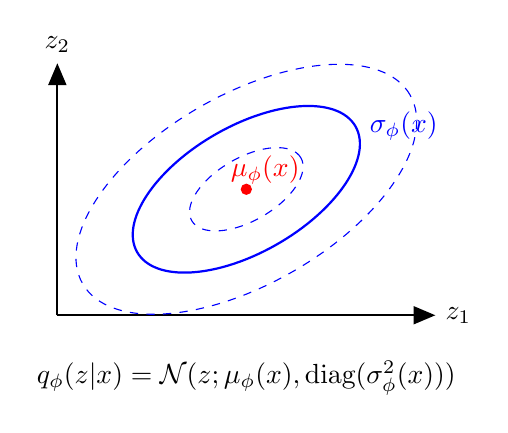
\begin{tikzpicture}[scale=0.8]
      % 2D Gaussian
      \draw[->,thick] (-3,-2) -- (3,-2) node[right] {$z_1$};
      \draw[->,thick] (-3,-2) -- (-3,2) node[above] {$z_2$};
      
      % Ellipse for Gaussian
      \draw[rotate=30,blue,thick] (0,0) ellipse (2 and 1);
      \draw[rotate=30,blue,dashed] (0,0) ellipse (1 and 0.5);
      \draw[rotate=30,blue,dashed] (0,0) ellipse (3 and 1.5);
      
      % Center point
      \filldraw[red] (0,0) circle (0.08);
      
      % Labels
      \node[red] at (0.3,0.3) {$\mu_\phi(x)$};
      \node[blue] at (2.5,1) {$\sigma_\phi(x)$};
      
      \node at (0,-3) {$q_\phi(z|x) = \mathcal{N}(z; \mu_\phi(x), \text{diag}(\sigma^2_\phi(x)))$};
    \end{tikzpicture}
      
    Encoder outputs:
        \begin{itemize}
          \item Mean vector: $\mu_\phi(x) \in \mathbb{R}^k$
          \item Log-variance: $\log \sigma^2_\phi(x) \in \mathbb{R}^k$
        \end{itemize}
  \end{columns}
\end{frame}




\begin{frame}{Mean Vector $\mu(x)$}
\begin{itemize}
\item $\mu(x) \in \mathbb{R}^k$ defines center of $q(z|x)$
\item Typically modeled by final layer of encoder network
\item No activation function (unbounded output)
\item Interpretable as "best guess" for latent code
\item Often carries most semantic information
\end{itemize}

\begin{center}
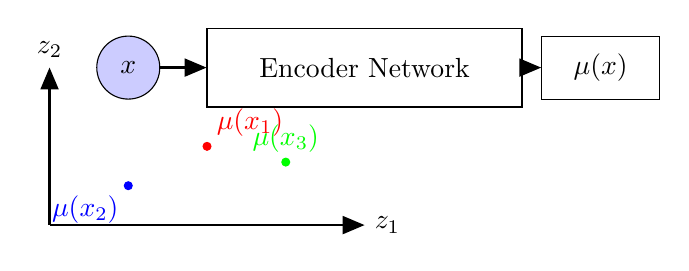
\begin{tikzpicture}
% Encoder outputs mean
\node[circle,draw,fill=blue!20,minimum size=0.8cm] (x) at (0,0) {$x$};
\node[rectangle,draw,minimum width=4cm,minimum height=1cm] (enc) at (3,0) {Encoder Network};
\node[rectangle,draw,minimum width=1.5cm,minimum height=0.8cm] (mu) at (6,0) {$\mu(x)$};
\draw[->,thick] (x) -- (enc);
\draw[->,thick] (enc) -- (mu);

% Visualization in 2D latent space
\draw[->,thick] (-1,-2) -- (3,-2) node[right] {$z_1$};
\draw[->,thick] (-1,-2) -- (-1,0) node[above] {$z_2$};
\filldraw[red] (1,-1) circle (0.05) node[above right] {$\mu(x_1)$};
\filldraw[blue] (0,-1.5) circle (0.05) node[below left] {$\mu(x_2)$};
\filldraw[green] (2,-1.2) circle (0.05) node[above] {$\mu(x_3)$};
\end{tikzpicture}
\end{center}
\end{frame}

\begin{frame}{Variance Vector $\sigma^2(x)$}
\begin{itemize}
\item $\sigma^2(x) \in \mathbb{R}^k$ defines uncertainty in $q(z|x)$
\item Network typically outputs $\log \sigma^2(x)$ for numerical stability
\item Apply $\exp$ to get positive variances
\item Larger variance = more uncertainty about latent code
\item Small variance = more confident encoding
\end{itemize}

\begin{center}
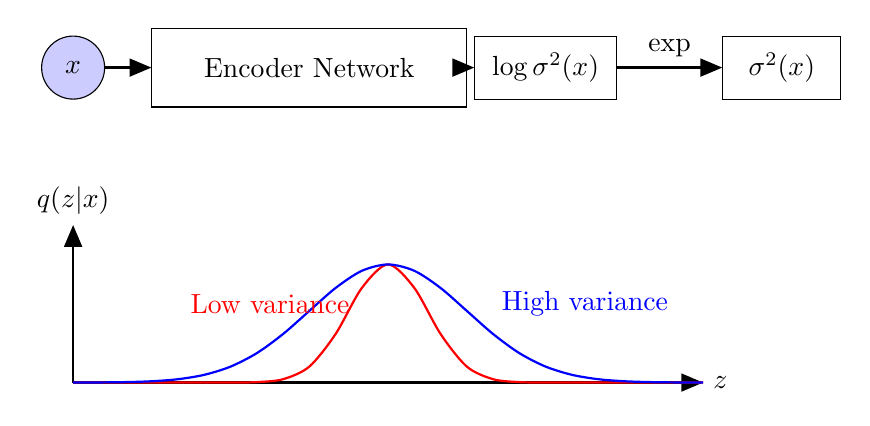
\begin{tikzpicture}
% Encoder outputs logvar
\node[circle,draw,fill=blue!20,minimum size=0.8cm] (x) at (0,0) {$x$};
\node[rectangle,draw,minimum width=4cm,minimum height=1cm] (enc) at (3,0) {Encoder Network};
\node[rectangle,draw,minimum width=1.8cm,minimum height=0.8cm] (logvar) at (6,0) {$\log\sigma^2(x)$};
\node[rectangle,draw,minimum width=1.5cm,minimum height=0.8cm] (var) at (9,0) {$\sigma^2(x)$};
\draw[->,thick] (x) -- (enc);
\draw[->,thick] (enc) -- (logvar);
\draw[->,thick] (logvar) -- (var) node[midway,above] {$\exp$};

% Uncertainty visualization in 1D
\draw[->,thick] (0,-4) -- (8,-4) node[right] {$z$};
\draw[->,thick] (0,-4) -- (0,-2) node[above] {$q(z|x)$};

\draw[domain=0:8, smooth, variable=\x, red, thick] 
  plot ({\x}, {-4+1.5*exp(-(\x-4)^2/0.5)});
\draw[domain=0:8, smooth, variable=\x, blue, thick] 
  plot ({\x}, {-4+1.5*exp(-(\x-4)^2/2.0)});

\node[red] at (2.5,-3) {Low variance};
\node[blue] at (6.5,-3) {High variance};
\end{tikzpicture}
\end{center}
\end{frame}


\begin{frame}

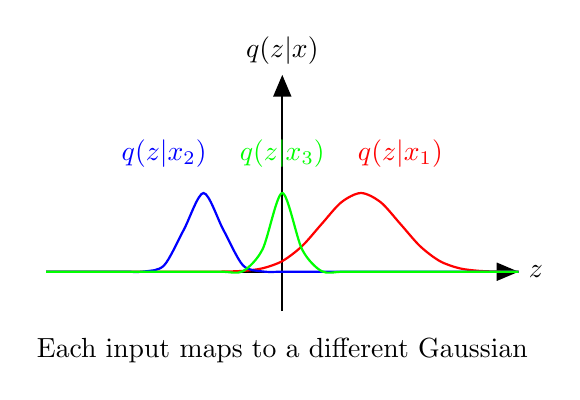
\begin{tikzpicture}
% Multiple Gaussians for different inputs
\draw[->,thick] (-3,0) -- (3,0) node[right] {$z$};
\draw[->,thick] (0,-0.5) -- (0,2.5) node[above] {$q(z|x)$};

 \draw[domain=-3:3, smooth, variable=\x, red, thick] 
   plot ({\x}, {exp(-(\x-1)^2/0.5)});
\draw[domain=-3:3, smooth, variable=\x, blue, thick] 
   plot ({\x}, {exp(-(\x+1)^2/0.1)});
\draw[domain=-3:3, smooth, variable=\x, green, thick] 
   plot ({\x}, {exp(-(\x)^2/0.05)});

\node[red] at (1.5,1.5) {$q(z|x_1)$};
\node[blue] at (-1.5,1.5) {$q(z|x_2)$};
\node[green] at (0,1.5) {$q(z|x_3)$};

\node at (0,-1) {Each input maps to a different Gaussian};
\end{tikzpicture}

    
\end{frame}


\begin{frame}{Sampling from $q(z|x)$}
\begin{itemize}
\item Need to sample $z \sim q(z|x)$ during training
\item Naively: $z \sim \mathcal{N}(\mu(x), \sigma^2(x))$
\item<2-> Problem: Sampling operation is not differentiable
\item<2-> Cannot backpropagate through random sampling
\item<3-> Solution: \textbf{Reparameterization trick}
\end{itemize}

\begin{center}
\only<2->{
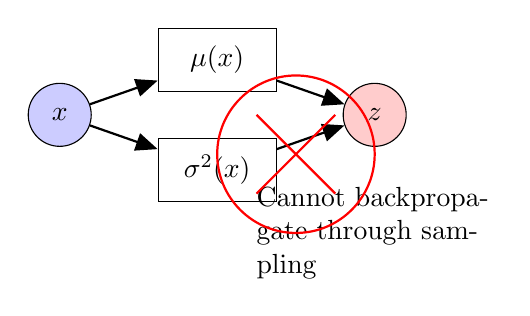
\begin{tikzpicture}
% Non-differentiable sampling
\node[circle,draw,fill=blue!20,minimum size=0.8cm] (x) at (0,0) {$x$};
\node[rectangle,draw,minimum width=1.5cm,minimum height=0.8cm] (mu) at (2,0.7) {$\mu(x)$};
\node[rectangle,draw,minimum width=1.5cm,minimum height=0.8cm] (var) at (2,-0.7) {$\sigma^2(x)$};
\node[circle,draw,fill=red!20,minimum size=0.8cm] (z) at (4,0) {$z$};
\draw[->,thick] (x) -- (mu);
\draw[->,thick] (x) -- (var);
\draw[->,thick] (mu) -- (z);
\draw[->,thick] (var) -- (z);
\node[text width=3cm] at (4,-1.5) {Cannot backpropagate through sampling};

% Problem symbol
\draw[red,thick] (3,-0.5) circle (1);
\draw[red,thick] (2.5,-1) -- (3.5,0);
\draw[red,thick] (2.5,0) -- (3.5,-1);
\end{tikzpicture}
}
\end{center}
\end{frame}




\begin{frame}{Reparameterization Trick - Intuition}
  \begin{columns}
    \column{0.6\textwidth}
    \begin{itemize}
      \item Challenge: We need to backpropagate through random sampling
      \item Problem: Random sampling isn't differentiable
      \item Solution: Reparameterization trick
        \begin{itemize}
          \item Express $z$ as a deterministic function of $x$ and some noise $\epsilon$
          \item Move randomness to an input that doesn't require gradients
        \end{itemize}
      \item Instead of sampling directly from $q_\phi(z|x)$:
        \begin{itemize}
          \item Sample $\epsilon \sim \mathcal{N}(0, I)$
          \item Compute $z = \mu_\phi(x) + \sigma_\phi(x) \odot \epsilon$
        \end{itemize}
      \item Now backpropagation works through $\mu_\phi(x)$ and $\sigma_\phi(x)$
    \end{itemize}
    
    \column{0.4\textwidth}
    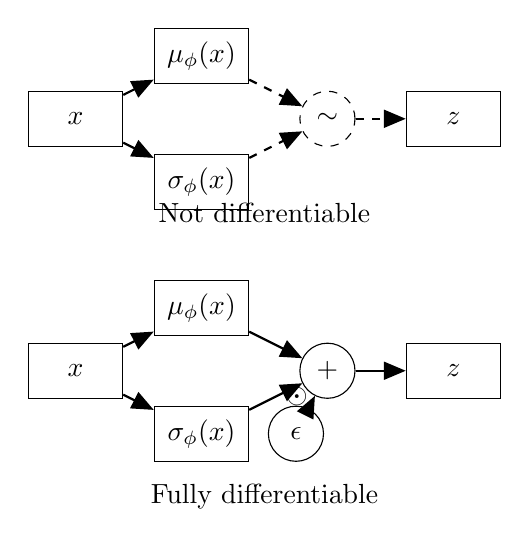
\begin{tikzpicture}[scale=0.8]
      % Before reparameterization
      \begin{scope}[shift={(0,2)}]
        \node[rectangle,draw,minimum width=1.2cm, minimum height=0.7cm] (x1) at (0,0) {$x$};
        \node[rectangle,draw,minimum width=1.2cm, minimum height=0.7cm] (mu1) at (2,1) {$\mu_\phi(x)$};
        \node[rectangle,draw,minimum width=1.2cm, minimum height=0.7cm] (sigma1) at (2,-1) {$\sigma_\phi(x)$};
        \node[circle,draw,dashed,minimum width=0.7cm] (sample1) at (4,0) {$\sim$};
        \node[rectangle,draw,minimum width=1.2cm, minimum height=0.7cm] (z1) at (6,0) {$z$};
        
        \draw[->,thick] (x1) -- (mu1);
        \draw[->,thick] (x1) -- (sigma1);
        \draw[->,thick,dashed] (mu1) -- (sample1);
        \draw[->,thick,dashed] (sigma1) -- (sample1);
        \draw[->,thick,dashed] (sample1) -- (z1);
        
        \node at (3,-1.5) {Not differentiable};
      \end{scope}
      
      % After reparameterization
      \begin{scope}[shift={(0,-2)}]
        \node[rectangle,draw,minimum width=1.2cm, minimum height=0.7cm] (x2) at (0,0) {$x$};
        \node[rectangle,draw,minimum width=1.2cm, minimum height=0.7cm] (mu2) at (2,1) {$\mu_\phi(x)$};
        \node[rectangle,draw,minimum width=1.2cm, minimum height=0.7cm] (sigma2) at (2,-1) {$\sigma_\phi(x)$};
        \node[circle,draw,minimum width=0.7cm] (epsilon) at (3.5,-1) {$\epsilon$};
        \node[circle,draw,minimum width=0.7cm] (add) at (4,0) {$+$};
        \node[rectangle,draw,minimum width=1.2cm, minimum height=0.7cm] (z2) at (6,0) {$z$};
        
        \draw[->,thick] (x2) -- (mu2);
        \draw[->,thick] (x2) -- (sigma2);
        \draw[->,thick] (mu2) -- (add);
        \draw[->,thick] (sigma2) -- node[midway,right] {$\odot$} (add);
        \draw[->,thick] (epsilon) -- (add);
        \draw[->,thick] (add) -- (z2);
        
        \node at (3,-2) {Fully differentiable};
      \end{scope}
    \end{tikzpicture}
  \end{columns}
\end{frame}


\begin{frame}{Mathematics of Reparameterization}
\begin{itemize}
\item Original formulation: $z \sim \mathcal{N}(\mu, \sigma^2)$
\item Reparameterized: $z = \mu + \sigma \odot \epsilon$, $\epsilon \sim \mathcal{N}(0, I)$
\item Equivalence proof:
  \begin{itemize}
  \item $\mathbb{E}[z] = \mathbb{E}[\mu + \sigma \odot \epsilon] = \mu + \sigma \odot \mathbb{E}[\epsilon] = \mu$
  \item $\text{Var}[z] = \text{Var}[\mu + \sigma \odot \epsilon] = \sigma^2 \odot \text{Var}[\epsilon] = \sigma^2$
  \end{itemize}
\end{itemize}

\begin{center}
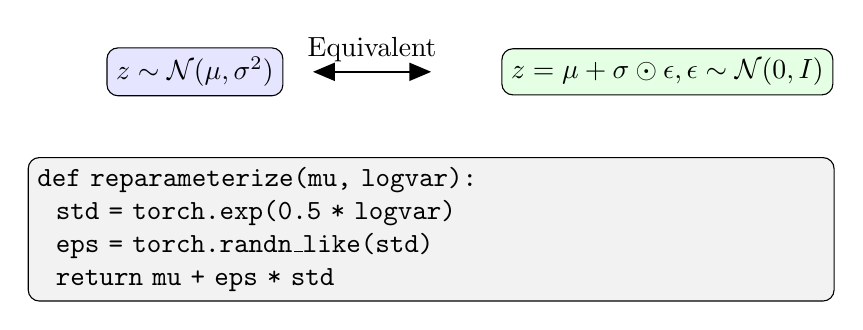
\begin{tikzpicture}
% Diagram showing equivalence
\node[rectangle,draw,fill=blue!10,rounded corners] at (0,0) {$z \sim \mathcal{N}(\mu, \sigma^2)$};
\node[rectangle,draw,fill=green!10,rounded corners] at (6,0) {$z = \mu + \sigma \odot \epsilon, \epsilon \sim \mathcal{N}(0, I)$};
\draw[<->,thick] (1.5,0) -- (3,0) node[midway,above] {Equivalent};

% Implementation code
\node[rectangle,draw,fill=gray!10,rounded corners,text width=10cm] at (3,-2) {
\texttt{def reparameterize(mu, logvar):}\\
\texttt{~~std = torch.exp(0.5 * logvar)}\\
\texttt{~~eps = torch.randn\_like(std)}\\
\texttt{~~return mu + eps * std}
};
\end{tikzpicture}
\end{center}
\end{frame}


\begin{frame}
    \centering
         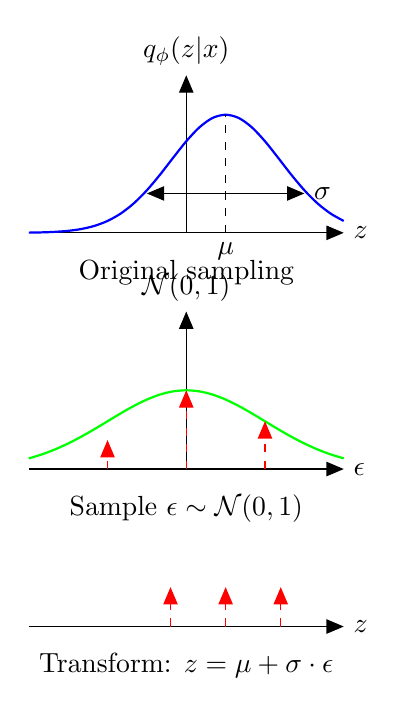
\begin{tikzpicture}[scale=1.0]
      % Original sampling
      \begin{scope}[shift={(0,2)}]
        \draw[->] (-2,0) -- (2,0) node[right] {$z$};
        \draw[->] (0,0) -- (0,2) node[above] {$q_\phi(z|x)$};
        \draw[domain=-2:2, smooth, variable=\x, blue, thick] 
          plot ({\x}, {1.5*exp(-(\x-0.5)^2/(2*0.7*0.7))});
        
        \draw[dashed] (0.5,0) -- (0.5,{1.5*exp(-(0.5-0.5)^2/(2*0.7*0.7))});
        \node[below] at (0.5,0) {$\mu$};
        
        \draw[<->] (-0.5,0.5) -- (1.5,0.5);
        \node[right] at (1.5,0.5) {$\sigma$};
        
        \node at (0,-0.5) {Original sampling};
      \end{scope}
      
      % Reparameterized sampling
      \begin{scope}[shift={(0,-1)}]
        \draw[->] (-2,0) -- (2,0) node[right] {$\epsilon$};
        \draw[->] (0,0) -- (0,2) node[above] {$\mathcal{N}(0,1)$};
        \draw[domain=-2:2, smooth, variable=\x, green, thick] 
          plot ({\x}, {exp(-\x*\x/2)});
        
        \draw[->, dashed, red] (-1,0) -- (-1,{exp(-1)});
        \draw[->, dashed, red] (0,0) -- (0,{exp(0)});
        \draw[->, dashed, red] (1,0) -- (1,{exp(-1/2)});
        
        \node at (0,-0.5) {Sample $\epsilon \sim \mathcal{N}(0,1)$};
      \end{scope}
      
      % Transformation
      \begin{scope}[shift={(0,-3)}]
        \draw[->] (-2,0) -- (2,0) node[right] {$z$};
        
        \draw[->, dashed, red] (-0.2,0) -- (-0.2,0.5);
        \draw[->, dashed, red] (0.5,0) -- (0.5,0.5);
        \draw[->, dashed, red] (1.2,0) -- (1.2,0.5);
        
        \node at (0,-0.5) {Transform: $z = \mu + \sigma \cdot \epsilon$};
      \end{scope}
    \end{tikzpicture}

    
\end{frame}


\begin{frame}{Enabling Backpropagation Through Stochastic Nodes}
  \begin{columns}
    \column{0.55\textwidth}
    \begin{itemize}
      \item Why is backpropagation challenging?
        \begin{itemize}
          \item Stochastic operations block gradient flow
          \item Sampling isn't differentiable
        \end{itemize}
      \item Reparameterization allows:
        \begin{itemize}
          \item Computing gradients w.r.t. $\mu_\phi(x)$ and $\sigma_\phi(x)$
          \item Optimizing encoder parameters $\phi$
          \item End-to-end training via back propagation 
        \end{itemize}
      \item Process:
        \begin{itemize}
          \item Forward pass: use reparameterization
          \item Backward pass: compute gradients through deterministic path
          \item Update parameters using gradient estimates
        \end{itemize}
    \end{itemize}
    
    \column{0.45\textwidth}
    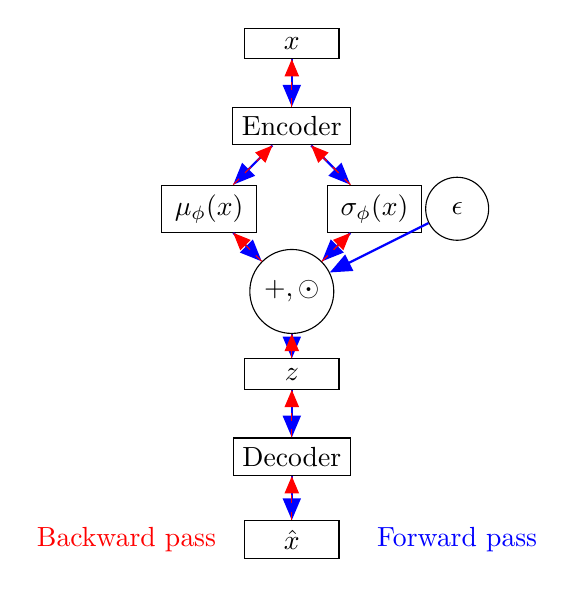
\begin{tikzpicture}[scale=0.7]
      % Computational graph
      \node[rectangle, draw, minimum width=1.2cm] (input) at (0,0) {$x$};
      \node[rectangle, draw, minimum width=1.2cm] (encoder) at (0,-1.5) {Encoder};
      \node[rectangle, draw, minimum width=1.2cm] (mu) at (-1.5,-3) {$\mu_\phi(x)$};
      \node[rectangle, draw, minimum width=1.2cm] (sigma) at (1.5,-3) {$\sigma_\phi(x)$};
      \node[circle, draw, minimum width=0.8cm] (epsilon) at (3,-3) {$\epsilon$};
      \node[circle, draw, minimum width=0.8cm] (reparam) at (0,-4.5) {$+,\odot$};
      \node[rectangle, draw, minimum width=1.2cm] (z) at (0,-6) {$z$};
      \node[rectangle, draw, minimum width=1.2cm] (decoder) at (0,-7.5) {Decoder};
      \node[rectangle, draw, minimum width=1.2cm] (output) at (0,-9) {$\hat{x}$};
      
      % Forward connections
      \draw[->, blue, thick] (input) -- (encoder);
      \draw[->, blue, thick] (encoder) -- (mu);
      \draw[->, blue, thick] (encoder) -- (sigma);
      \draw[->, blue, thick] (mu) -- (reparam);
      \draw[->, blue, thick] (sigma) -- (reparam);
      \draw[->, blue, thick] (epsilon) -- (reparam);
      \draw[->, blue, thick] (reparam) -- (z);
      \draw[->, blue, thick] (z) -- (decoder);
      \draw[->, blue, thick] (decoder) -- (output);
      
      % Backward connections
      \draw[->, red, dashed] (output) -- (decoder);
      \draw[->, red, dashed] (decoder) -- (z);
      \draw[->, red, dashed] (z) -- (reparam);
      \draw[->, red, dashed] (reparam) -- (mu);
      \draw[->, red, dashed] (reparam) -- (sigma);
      \draw[->, red, dashed] (mu) -- (encoder);
      \draw[->, red, dashed] (sigma) -- (encoder);
      \draw[->, red, dashed] (encoder) -- (input);
      
      % Labels
      \node[blue] at (3,-9) {Forward pass};
      \node[red] at (-3,-9) {Backward pass};
    \end{tikzpicture}
  \end{columns}
\end{frame}


\begin{frame}{Decoder Network - Overview}
\begin{itemize}
\item Maps latent code $z$ to parameters of $p(x|z)$
\item Mirror of encoder architecture (typically)
\item Input: latent vector $z \in \mathbb{R}^k$
\item Output: parameters for data distribution $p(x|z)$
\item Training objective: maximize $\log p(x|z)$
\end{itemize}

\begin{center}
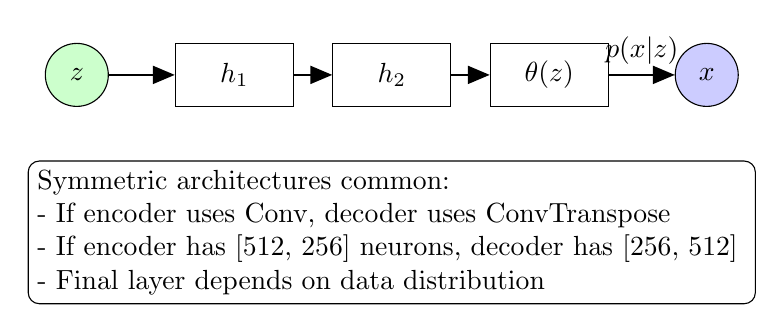
\begin{tikzpicture}
% Decoder network
\node[circle,draw,fill=green!20,minimum size=0.8cm] (z) at (0,0) {$z$};
\node[rectangle,draw,minimum width=1.5cm,minimum height=0.8cm] (h1) at (2,0) {$h_1$};
\node[rectangle,draw,minimum width=1.5cm,minimum height=0.8cm] (h2) at (4,0) {$h_2$};
\node[rectangle,draw,minimum width=1.5cm,minimum height=0.8cm] (out) at (6,0) {$\theta(z)$};
\node[circle,draw,fill=blue!20,minimum size=0.8cm] (x) at (8,0) {$x$};

\draw[->,thick] (z) -- (h1);
\draw[->,thick] (h1) -- (h2);
\draw[->,thick] (h2) -- (out);
\draw[->,thick] (out) -- (x) node[midway,above] {$p(x|z)$};

% Architecture examples
\node[draw,rounded corners,text width=9cm] at (4,-2) {
Symmetric architectures common:\\
- If encoder uses Conv, decoder uses ConvTranspose\\
- If encoder has [512, 256] neurons, decoder has [256, 512]\\
- Final layer depends on data distribution
};
\end{tikzpicture}
\end{center}
\end{frame}




\begin{frame}{Mapping $z \to p(x|z)$ | Bernoulli Likelihood}
\begin{itemize}
\item For binary data: $p(x|z) = \text{Bernoulli}(x; \theta(z))$
\item $\theta(z) \in [0,1]^d$ is probability of each bit being 1
\item Final decoder layer uses sigmoid activation: $\sigma(a) = \frac{1}{1+e^{-a}}$
\item Negative log-likelihood = binary cross-entropy loss
\item $-\log p(x|z) = -\sum_i [x_i \log \theta_i(z) + (1-x_i) \log (1-\theta_i(z))]$
\item Example use cases:
\begin{itemize}
    \item MNIST Digit (0/1 pixels)
    \item Text data (Tokenised and 0/1 for each token)
    
\end{itemize}
\end{itemize}

\end{frame}


\begin{frame}{Mapping $z \to p(x|z)$ | Gaussian Likelihood}
\begin{itemize}
\item For continuous data: $p(x|z) = \mathcal{N}(x; \mu(z), \sigma^2(z))$
\item Decoder outputs mean $\mu(z)$ (no activation) and log-variance $\log \sigma^2(z)$
\item Fixed variance simplification: $p(x|z) = \mathcal{N}(x; \mu(z), \sigma^2 I)$
\item With fixed $\sigma^2$, negative log-likelihood $\propto$ MSE
\item $-\log p(x|z) \propto \frac{1}{2\sigma^2}\|x - \mu(z)\|^2$
\item Example use cases:
\begin{itemize}
    \item Natural images (pixel values)
    \item Audio Waveforms
\end{itemize}

\end{itemize}

\end{frame}


\begin{frame}{Sampling from VAE}
\begin{itemize}
\item To generate new samples:
  \begin{enumerate}
  \item Sample $z \sim \mathcal{N}(0, I)$ from prior
  \item Decode $z$ using the decoder: $x \sim p(x|z)$
  \end{enumerate}
\item For Bernoulli outputs:
  \begin{itemize}
  \item Either sample from $\text{Bernoulli}(\theta(z))$
  \item Or use thresholded probabilities: $x_i = [\theta_i(z) > 0.5]$
  \end{itemize}
\item For Gaussian outputs: sample or use mean
\end{itemize}

\begin{center}
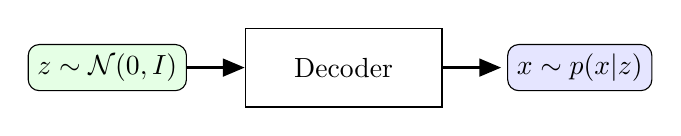
\begin{tikzpicture}
% Sampling process
\node[rectangle,draw,fill=green!10,rounded corners] at (0,0) {$z \sim \mathcal{N}(0, I)$};
\node[rectangle,draw,minimum width=2.5cm,minimum height=1cm] (dec) at (3,0) {Decoder};
\node[rectangle,draw,fill=blue!10,rounded corners] at (6,0) {$x \sim p(x|z)$};
\draw[->,thick] (1,0) -- (dec);
\draw[->,thick] (dec) -- (5,0);

\end{tikzpicture}
\end{center}
\end{frame}


\begin{frame}{Interpolation in Latent Space}
\begin{itemize}
\item Smooth traversal between two points in latent space
\item For two inputs $x_1, x_2$:
  \begin{enumerate}
  \item Encode: $z_1 = \mu(x_1)$, $z_2 = \mu(x_2)$
  \item Interpolate: $z_t = (1-t) \cdot z_1 + t \cdot z_2$, $t \in [0, 1]$
  \item Decode: $x_t \sim p(x|z_t)$
  \end{enumerate}
\item Creates smooth morphing between inputs
\item Reveals latent space structure
\end{itemize}

\begin{center}
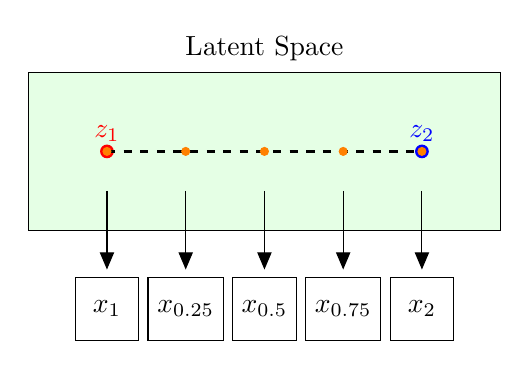
\begin{tikzpicture}
% Latent space interpolation
\draw[fill=green!10] (-3,-1) rectangle (3,1);
\node at (0,1.3) {Latent Space};

% Two points
\filldraw[red] (-2,0) circle (0.08) node[above] {$z_1$};
\filldraw[blue] (2,0) circle (0.08) node[above] {$z_2$};

% Interpolation
\draw[thick,dashed] (-2,0) -- (2,0);
\foreach \i in {0,0.25,0.5,0.75,1} {
  \pgfmathsetmacro{\x}{-2+4*\i}
  \filldraw[orange] (\x,0) circle (0.05);
}

% Images
\node[rectangle,draw,minimum width=0.8cm,minimum height=0.8cm] at (-2,-2) {$x_1$};
\node[rectangle,draw,minimum width=0.8cm,minimum height=0.8cm] at (-1,-2) {$x_{0.25}$};
\node[rectangle,draw,minimum width=0.8cm,minimum height=0.8cm] at (0,-2) {$x_{0.5}$};
\node[rectangle,draw,minimum width=0.8cm,minimum height=0.8cm] at (1,-2) {$x_{0.75}$};
\node[rectangle,draw,minimum width=0.8cm,minimum height=0.8cm] at (2,-2) {$x_2$};

\draw[->] (-2,-0.5) -- (-2,-1.5);
\draw[->] (-1,-0.5) -- (-1,-1.5);
\draw[->] (0,-0.5) -- (0,-1.5);
\draw[->] (1,-0.5) -- (1,-1.5);
\draw[->] (2,-0.5) -- (2,-1.5);
\end{tikzpicture}
\end{center}
\end{frame}

\begin{frame}{Network Architectures - Fully Connected}
\begin{itemize}
\item Simplest architecture: Multi-Layer Perceptron (MLP)
\item Encoder: flattened input $\to$ FC layers $\to$ $\mu, \log\sigma^2$
\item Decoder: latent $z$ $\to$ FC layers $\to$ reshaped output
\item Suitable for:
  \begin{itemize}
  \item Low-dimensional data
  \item Data without spatial structure
  \item Proof-of-concept implementations
  \end{itemize}
\end{itemize}

\begin{center}
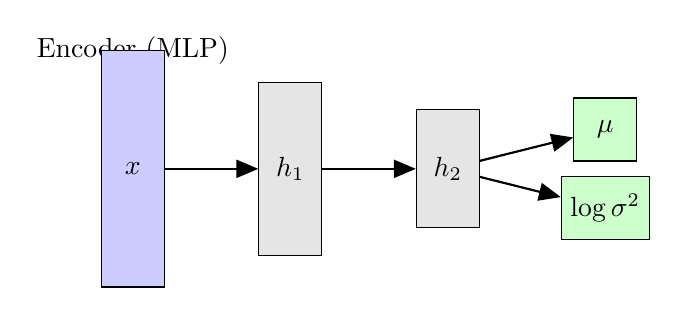
\begin{tikzpicture}
% Encoder MLP
\node at (0,1.5) {Encoder (MLP)};
\node[rectangle,draw,fill=blue!20,minimum width=0.8cm,minimum height=3cm] (in) at (0,0) {$x$};
\node[rectangle,draw,fill=gray!20,minimum width=0.8cm,minimum height=2.2cm] (h1) at (2,0) {$h_1$};
\node[rectangle,draw,fill=gray!20,minimum width=0.8cm,minimum height=1.5cm] (h2) at (4,0) {$h_2$};
\node[rectangle,draw,fill=green!20,minimum width=0.8cm,minimum height=0.8cm] (mu) at (6,0.5) {$\mu$};
\node[rectangle,draw,fill=green!20,minimum width=0.8cm,minimum height=0.8cm] (logvar) at (6,-0.5) {$\log\sigma^2$};

\draw[->,thick] (in) -- (h1);
\draw[->,thick] (h1) -- (h2);
\draw[->,thick] (h2) -- (mu);
\draw[->,thick] (h2) -- (logvar);


\end{tikzpicture}
\end{center}
\end{frame}

\begin{frame}{Network Architectures - Convolutional}
\begin{itemize}
\item CNN-based architecture for images and spatial data
\item Encoder: Conv layers $\to$ flatten $\to$ FC $\to$ $\mu, \log\sigma^2$
\item Decoder: $z$ $\to$ FC $\to$ reshape $\to$ ConvTranspose layers
\item Benefits:
  \begin{itemize}
  \item Parameter sharing
  \item Translation invariance
  \item Better spatial representation
  \end{itemize}
\end{itemize}
\end{frame}


\begin{frame}

\begin{center}
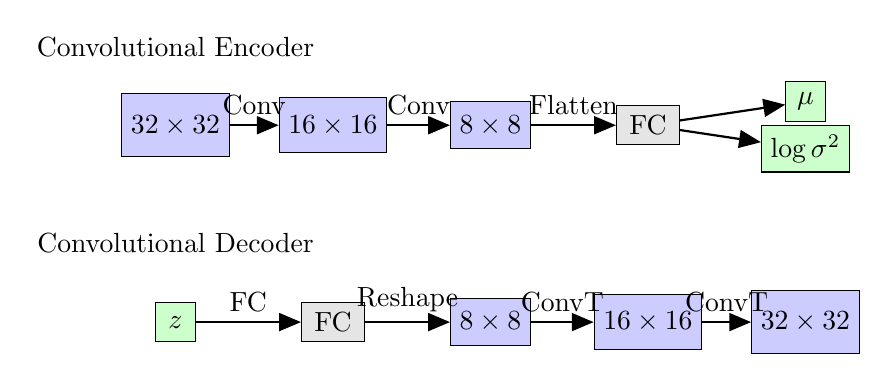
\begin{tikzpicture}
% Convolutional VAE
\node at (0,2) {Convolutional Encoder};
\node[rectangle,draw,fill=blue!20,minimum width=0.8cm,minimum height=0.8cm] (in) at (0,1) {$32 \times 32$};
\node[rectangle,draw,fill=blue!20,minimum width=0.7cm,minimum height=0.7cm] (c1) at (2,1) {$16 \times 16$};
\node[rectangle,draw,fill=blue!20,minimum width=0.6cm,minimum height=0.6cm] (c2) at (4,1) {$8 \times 8$};
\node[rectangle,draw,fill=gray!20,minimum width=0.8cm,minimum height=0.5cm] (fc) at (6,1) {FC};
\node[rectangle,draw,fill=green!20,minimum width=0.5cm,minimum height=0.5cm] (mu) at (8,1.3) {$\mu$};
\node[rectangle,draw,fill=green!20,minimum width=0.5cm,minimum height=0.5cm] (logvar) at (8,0.7) {$\log\sigma^2$};

\draw[->,thick] (in) -- node[above] {Conv} (c1);
\draw[->,thick] (c1) -- node[above] {Conv} (c2);
\draw[->,thick] (c2) -- node[above] {Flatten} (fc);
\draw[->,thick] (fc) -- (mu);
\draw[->,thick] (fc) -- (logvar);

% Decoder
\node at (0,-0.5) {Convolutional Decoder};
\node[rectangle,draw,fill=green!20,minimum width=0.5cm,minimum height=0.5cm] (z) at (0,-1.5) {$z$};
\node[rectangle,draw,fill=gray!20,minimum width=0.8cm,minimum height=0.5cm] (fc2) at (2,-1.5) {FC};
\node[rectangle,draw,fill=blue!20,minimum width=0.6cm,minimum height=0.6cm] (d1) at (4,-1.5) {$8 \times 8$};
\node[rectangle,draw,fill=blue!20,minimum width=0.7cm,minimum height=0.7cm] (d2) at (6,-1.5) {$16 \times 16$};
\node[rectangle,draw,fill=blue!20,minimum width=0.8cm,minimum height=0.8cm] (out) at (8,-1.5) {$32 \times 32$};

\draw[->,thick] (z) -- node[above] {FC} (fc2);
\draw[->,thick] (fc2) -- node[above] {Reshape} (d1);
\draw[->,thick] (d1) -- node[above] {ConvT} (d2);
\draw[->,thick] (d2) -- node[above] {ConvT} (out);
\end{tikzpicture}
\end{center}
    
\end{frame}

\begin{frame}{Activation Functions}
\begin{itemize}
\item Common choices for hidden layers:
  \begin{itemize}
  \item ReLU: $f(x) = \max(0, x)$ - Most common
  \item LeakyReLU: $f(x) = \max(0.01x, x)$ - Prevents dead neurons
  \item Tanh: $f(x) = \tanh(x)$ - Bounded output
  \end{itemize}
\item Output layer activation:
  \begin{itemize}
  \item Mean $\mu(x)$, $\mu(z)$: None (linear)
  \item Log-variance $\log\sigma^2$: None (linear)
  \item Bernoulli parameter $\theta(z)$: Sigmoid
  \end{itemize}
\end{itemize}

\begin{center}
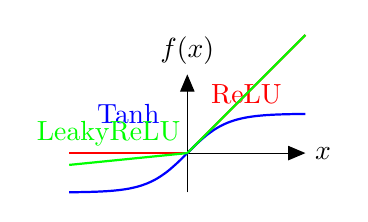
\begin{tikzpicture}[scale=0.5]
% Plot axes
\draw[->] (-3,0) -- (3,0) node[right] {$x$};
\draw[->] (0,-1) -- (0,2) node[above] {$f(x)$};

% ReLU
\draw[domain=-3:0, smooth, variable=\x, red, thick] plot ({\x}, {0});
\draw[domain=0:3, smooth, variable=\x, red, thick] plot ({\x}, {\x});
\node[red] at (1.5,1.5) {ReLU};

% Tanh
\draw[domain=-3:3, smooth, variable=\x, blue, thick] plot ({\x}, {tanh(\x)});
\node[blue] at (-1.5,1) {Tanh};

% LeakyReLU
\draw[domain=-3:0, smooth, variable=\x, green, thick] plot ({\x}, {0.1*\x});
\draw[domain=0:3, smooth, variable=\x, green, thick] plot ({\x}, {\x});
\node[green] at (-2,0.5) {LeakyReLU};
\end{tikzpicture}
\end{center}
\end{frame}

\begin{frame}{Implementation Considerations}
\begin{itemize}
\item \textbf{Balancing encoder/decoder capacity}:
  \begin{itemize}
  \item Symmetric architectures often work well
  \item Decoder may need more capacity for complex data
  \end{itemize}
\item \textbf{Latent dimension selection}:
  \begin{itemize}
  \item Too small: poor reconstruction
  \item Too large: may not learn good representations
  \item Typical values: 2-10 (visualization), 32-256 (performance)
  \end{itemize}
\item \textbf{Training strategies}:
  \begin{itemize}
  \item Consider KL annealing for complex data
  \item Monitor both loss components separately
  \item Use gradient clipping if training unstable
  \end{itemize}
\end{itemize}

\begin{center}
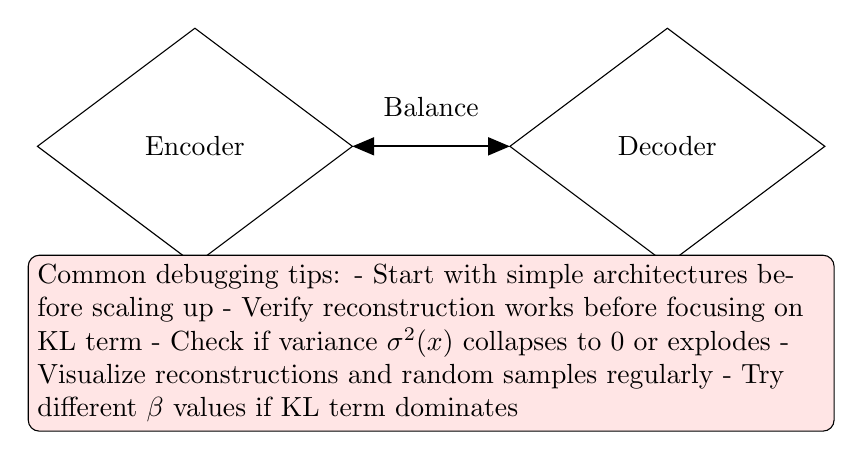
\begin{tikzpicture}
% Balancing capacity
\draw (0,0) -- (2,1.5) -- (4,0) -- (2,-1.5) -- cycle;
\node at (2,0) {Encoder};

\draw (6,0) -- (8,1.5) -- (10,0) -- (8,-1.5) -- cycle;
\node at (8,0) {Decoder};

\draw[<->,thick] (4,0) -- (6,0);
\node at (5,0.5) {Balance};

% Debug tips
\node[rectangle,draw,fill=red!10,rounded corners,text width=10cm] at (5,-2.5) {
Common debugging tips:
- Start with simple architectures before scaling up
- Verify reconstruction works before focusing on KL term
- Check if variance $\sigma^2(x)$ collapses to 0 or explodes
- Visualize reconstructions and random samples regularly
- Try different $\beta$ values if KL term dominates
};
\end{tikzpicture}
\end{center}
\end{frame}


%%%%%%%%%%%%%%%%%%%%%%%%%%%%%%%%%%%%%%%%%%%%%%%%%%%%%%%%%%%%%%%%%%%%%%%
% Section 3.3: Loss Functions & Reconstruction Quality (40 minutes)
%%%%%%%%%%%%%%%%%%%%%%%%%%%%%%%%%%%%%%%%%%%%%%%%%%%%%%%%%%%%%%%%%%%%%%%



\section{Loss Functions \& Reconstruction Quality}

\begin{frame}{Loss Functions \& Reconstruction Quality}
\begin{itemize}
\item Evidence Lower Bound (ELBO) intuition ( and derivation)
\item Reconstruction loss term and variants
\item KL divergence regularization
\item Balancing reconstruction and regularization
\item $\beta$-VAE and disentanglement
\item Common pitfalls and solutions
\item Practical training strategies
\end{itemize}

\begin{center}
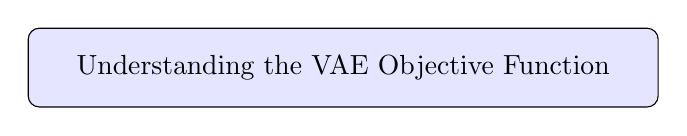
\begin{tikzpicture}
\node[rectangle,draw,fill=blue!10,rounded corners,minimum width=8cm,minimum height=1cm] at (0,0) {Understanding the VAE Objective Function};
\end{tikzpicture}
\end{center}
\end{frame}


\begin{frame}{Evidence Lower Bound (ELBO) - Intuition}
\begin{itemize}
\item Goal: Maximize data log-likelihood $\log p(x)$
\item Challenge: $p(x) = \int p(x|z)p(z)dz$ is intractable
\item Solution: Derive a lower bound on $\log p(x)$ that we can optimize
\item Variational inference: Approximate true posterior $p(z|x)$ with $q(z|x)$
\item ELBO: $\log p(x) \geq \mathbb{E}_{q(z|x)}[\log p(x|z)] - D_{KL}(q(z|x) \| p(z))$
\end{itemize}

\begin{center}
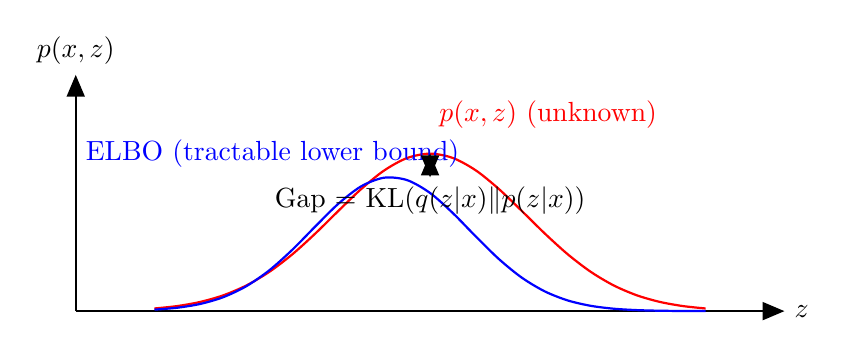
\begin{tikzpicture}
% Visualization of lower bound
\draw[->,thick] (0,0) -- (9,0) node[right] {$z$};
\draw[->,thick] (0,0) -- (0,3) node[above] {$p(x,z)$};

% True distribution (unknown)
\draw[domain=1:8, smooth, variable=\x, red, thick] 
  plot ({\x}, {2*exp(-(\x-4.5)^2/3)});
\node[red] at (6,2.5) {$p(x,z)$ (unknown)};

% Lower bound
\draw[domain=1:8, smooth, variable=\x, blue, thick] 
  plot ({\x}, {1.7*exp(-(\x-4)^2/2)});
\node[blue] at (2.5,2) {ELBO (tractable lower bound)};

% Gap
\draw[<->,thick,dashed] (4.5,1.7) -- (4.5,2);
\node at (4.5,1.4) {Gap = KL($q(z|x) \| p(z|x)$)};
\end{tikzpicture}
\end{center}
\end{frame}

\begin{frame}{Reconstruction Loss Term}
\begin{itemize}
\item First term in ELBO: $\mathbb{E}_{q(z|x)}[\log p(x|z)]$
\item Interpretation: How well can we reconstruct $x$ from its latent encoding?
\item Depends on form of $p(x|z)$ (likelihood function)
\item Monte Carlo estimation with reparameterization:
  \begin{itemize}
  \item Sample $\epsilon \sim \mathcal{N}(0, I)$
  \item Compute $z = \mu(x) + \sigma(x) \odot \epsilon$
  \item Evaluate $\log p(x|z)$
  \end{itemize}
\item Typically, a single sample is used during training
\end{itemize}

\begin{center}
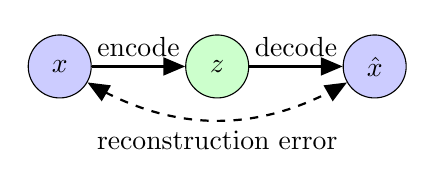
\begin{tikzpicture}
% Visual representation
\node[circle,draw,fill=blue!20,minimum size=0.8cm] (x1) at (0,0) {$x$};
\node[circle,draw,fill=green!20,minimum size=0.8cm] (z1) at (2,0) {$z$};
\node[circle,draw,fill=blue!20,minimum size=0.8cm] (x2) at (4,0) {$\hat{x}$};

\draw[->,thick] (x1) -- node[above] {encode} (z1);
\draw[->,thick] (z1) -- node[above] {decode} (x2);
\draw[<->,thick,dashed] (x1) to[bend right] node[below] {reconstruction error} (x2);
\end{tikzpicture}

\end{center}
\end{frame}

\begin{frame}
\centering
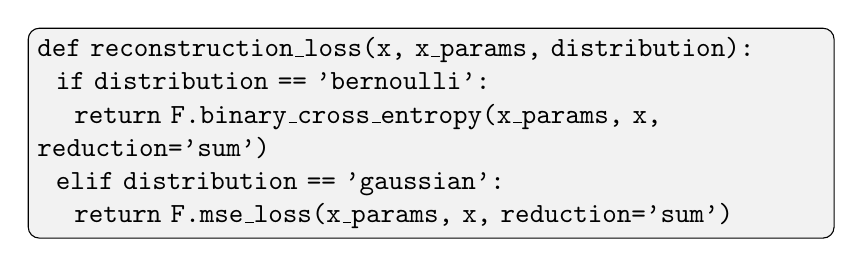
\begin{tikzpicture}
    % Code implementation
\node[rectangle,draw,fill=gray!10,rounded corners,text width=10cm] at (2,-2) {
\texttt{def reconstruction\_loss(x, x\_params, distribution):}\\
\texttt{~~if distribution == 'bernoulli':}\\
\texttt{~~~~return F.binary\_cross\_entropy(x\_params, x, reduction='sum')}\\
\texttt{~~elif distribution == 'gaussian':}\\
\texttt{~~~~return F.mse\_loss(x\_params, x, reduction='sum')}
};
\end{tikzpicture}

    
\end{frame}


\begin{frame}{Binary Cross-Entropy vs. Mean-Squared Error}
  \begin{center}
    \begin{tabular}{p{7cm}|p{7cm}}
      \toprule
      \textbf{Binary Cross-Entropy} & \textbf{Mean-Squared Error} \\
      \midrule
      Derived from Bernoulli likelihood & Derived from Gaussian likelihood \\
      \midrule
      Better for binary data & Better for continuous data \\
      \midrule
      $-\sum_i [x_i \log(\hat{x}_i) + (1-x_i)\log(1-\hat{x}_i)]$ & $\sum_i (x_i - \hat{x}_i)^2$ \\
      \midrule
      Strong penalty for confident wrong predictions & Uniform penalty based on distance\\
      \midrule
      Common for MNIST, binary images & Common for natural images, audio \\
      \midrule
      Often used with sigmoid output & Often used with linear/tanh output \\
      \bottomrule
    \end{tabular}
  \end{center}

\end{frame}


\begin{frame}{KL Divergence Term}
\begin{itemize}
\item Second term in ELBO: $-D_{KL}(q(z|x) \| p(z))$
\item Measures how much $q(z|x)$ differs from prior $p(z)$
\item Penalizes complex encodings that diverge from prior
\item Functions as a regularizer that:
  \begin{itemize}
  \item Prevents overfitting
  \item Encourages use of all latent dimensions
  \item Creates a smooth, continuous latent space
  \item Enables sampling from the prior
  \end{itemize}
\end{itemize}
\end{frame}

\begin{frame}{KL Divergence: Measuring Distribution Difference}

\textbf{What is KL Divergence?}
\begin{itemize}
    \item \textbf{Kullback-Leibler (KL) divergence} quantifies how one probability distribution diverges from a second, expected distribution.
    \item In VAEs, it measures how much the approximate posterior $q(z|x)$ differs from the prior $p(z)$.
\end{itemize}

\vspace{2mm}
\textbf{Mathematical Definition:}
\[
D_{KL}(q(z|x) \| p(z)) = \int q(z|x) \log \frac{q(z|x)}{p(z)} dz
\]

\vspace{2mm}
\textbf{Key Properties:}
\begin{itemize}
    \item $D_{KL}(q \| p) \geq 0$ (always non-negative)
    \item $D_{KL}(q \| p) = 0$ if and only if $q = p$ almost everywhere
    \item \textbf{Asymmetric:} $D_{KL}(q \| p) \neq D_{KL}(p \| q)$
\end{itemize}



\end{frame}

\begin{frame}{KL Divergence: Measuring Distribution Difference}
\vspace{2mm}
\textbf{Intuition:}
\begin{itemize}
    \item KL divergence is \textit{not} a true distance, but a measure of information loss when $p$ is used to approximate $q$.
    \item In VAEs, minimizing KL ensures the learned latent codes ($q(z|x)$) stay close to the prior ($p(z)$), promoting smoothness and generative ability.
\end{itemize}

\begin{center}
\begin{columns}

    \begin{column}{0.5\textwidth}
    \centering
    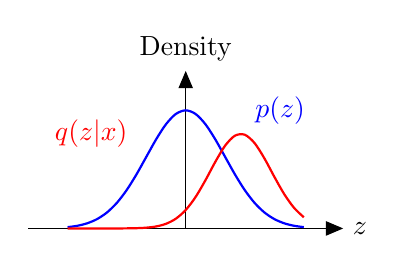
\begin{tikzpicture}
    % Axes
    \draw[->] (-2,0) -- (2,0) node[right] {$z$};
    \draw[->] (0,0) -- (0,2) node[above] {Density};
    % Prior
    \draw[domain=-1.5:1.5,smooth,variable=\x,blue,thick] plot ({\x},{1.5*exp(-(\x)^2/0.5)});
    \node[blue] at (1.2,1.5) {$p(z)$};
    % Posterior
    \draw[domain=-1.5:1.5,smooth,variable=\x,red,thick] plot ({\x},{1.2*exp(-(\x-0.7)^2/0.3)});
    \node[red] at (-1.2,1.2) {$q(z|x)$};
    \end{tikzpicture}
    \end{column}
    \begin{column}{0.5\textwidth}
    \centering
    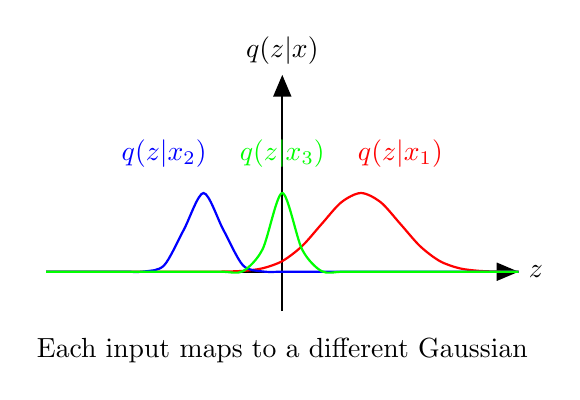
\begin{tikzpicture}
% Multiple Gaussians for different inputs
\draw[->,thick] (-3,0) -- (3,0) node[right] {$z$};
\draw[->,thick] (0,-0.5) -- (0,2.5) node[above] {$q(z|x)$};

 \draw[domain=-3:3, smooth, variable=\x, red, thick] 
   plot ({\x}, {exp(-(\x-1)^2/0.5)});
\draw[domain=-3:3, smooth, variable=\x, blue, thick] 
   plot ({\x}, {exp(-(\x+1)^2/0.1)});
\draw[domain=-3:3, smooth, variable=\x, green, thick] 
   plot ({\x}, {exp(-(\x)^2/0.05)});

\node[red] at (1.5,1.5) {$q(z|x_1)$};
\node[blue] at (-1.5,1.5) {$q(z|x_2)$};
\node[green] at (0,1.5) {$q(z|x_3)$};

\node at (0,-1) {Each input maps to a different Gaussian};
\end{tikzpicture}
    \end{column}
\end{columns}

\end{center}
    
\end{frame}

\begin{frame}{KL Divergence in VAEs: General and Gaussian Case}

\textbf{General Definition:}
\[
D_{KL}(q(z|x) \| p(z)) = \int q(z|x) \log \frac{q(z|x)}{p(z)} dz
\]

\vspace{2mm}
\textbf{In VAEs:}
\begin{itemize}
    \item $q(z|x)$: Encoder's approximate posterior (usually Gaussian)
    \item $p(z)$: Prior (often standard normal)
    \item KL term regularizes $q(z|x)$ to stay close to $p(z)$
\end{itemize}

\vspace{2mm}
\textbf{Closed-Form for Standard Gaussian Prior:}
\begin{itemize}
    \item If $q(z|x) = \mathcal{N}(\mu, \mathrm{diag}(\sigma^2))$ and $p(z) = \mathcal{N}(0, I)$:
\end{itemize}
\[
D_{KL}(q(z|x) \| p(z)) = \frac{1}{2} \sum_{i=1}^d \left( \mu_i^2 + \sigma_i^2 - \log \sigma_i^2 - 1 \right)
\]

\vspace{2mm}
\textbf{Interpretation:}
\begin{itemize}
    \item Penalizes $\mu_i$ far from $0$ (prior mean)
    \item Penalizes $\sigma_i^2$ far from $1$ (prior variance)
    \item Encourages $q(z|x)$ to match $p(z)$ for all $x$
\end{itemize}

\begin{center}
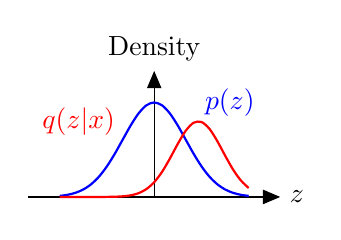
\begin{tikzpicture}[scale=0.8]
    % Axes
    \draw[->] (-2,0) -- (2,0) node[right] {$z$};
    \draw[->] (0,0) -- (0,2) node[above] {Density};
    % Prior
    \draw[domain=-1.5:1.5,smooth,variable=\x,blue,thick] plot ({\x},{1.5*exp(-(\x)^2/0.5)});
    \node[blue] at (1.2,1.5) {$p(z)$};
    % Posterior
    \draw[domain=-1.5:1.5,smooth,variable=\x,red,thick] plot ({\x},{1.2*exp(-(\x-0.7)^2/0.3)});
    \node[red] at (-1.2,1.2) {$q(z|x)$};
\end{tikzpicture}
\end{center}

\end{frame}

\begin{frame}{Latent Space Regularization}
\begin{itemize}
\item Why regularize towards prior $p(z)$?
  \begin{itemize}
  \item Creates a well-structured latent space
  \item Allows interpolation between points
  \item Enables sampling from the prior
  \item Prevents overfitting to training data
  \end{itemize}
\item Without KL, model becomes a deterministic autoencoder
\item With too much KL, reconstructions are poor
\item Finding the right balance is critical
\end{itemize}


\end{frame}

\begin{frame}{$\beta$-VAE and Disentanglement}
\begin{itemize}
\item Modified ELBO with hyperparameter $\beta$:
\begin{align}
\mathcal{L}(\theta, \phi; x, \beta) = \mathbb{E}_{q(z|x)}[\log p(x|z)] - \beta \cdot D_{KL}(q(z|x) \| p(z))
\end{align}
\item $\beta = 1$: Standard VAE
\item $\beta < 1$: Focus on better reconstruction
\item $\beta > 1$: Stronger regularization, better disentanglement
\item Disentanglement: Independent factors in latent space
\end{itemize}


\end{frame}

\begin{frame}

\begin{center}
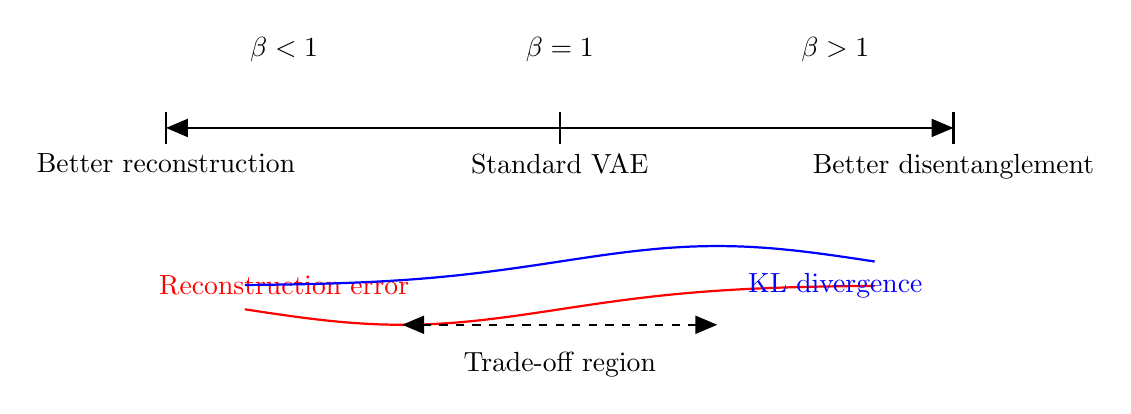
\begin{tikzpicture}
% Beta values visualization
\node at (-3.5,1) {$\beta < 1$};
\node at (0,1) {$\beta = 1$};
\node at (3.5,1) {$\beta > 1$};

\draw[<->,thick] (-5,0) -- (5,0);
\draw[thick] (-5,0.2) -- (-5,-0.2) node[below] {Better reconstruction};
\draw[thick] (5,0.2) -- (5,-0.2) node[below] {Better disentanglement};
\draw[thick] (0,0.2) -- (0,-0.2) node[below] {Standard VAE};

% Trade-off curves
\draw[domain=-4:4, smooth, variable=\x, red, thick] 
  plot ({\x}, {-2-0.5*exp(-(\x+2)*(\x+2)/8)});
\node[red] at (-3.5,-2) {Reconstruction error};

\draw[domain=-4:4, smooth, variable=\x, blue, thick] 
  plot ({\x}, {-2+0.5*exp(-(\x-2)*(\x-2)/8)});
\node[blue] at (3.5,-2) {KL divergence};

\draw[<->,thick,dashed] (-2,-2.5) -- (2,-2.5);
\node at (0,-3) {Trade-off region};
\end{tikzpicture}
\end{center}
    
\end{frame}


\begin{frame}{Common Pitfall: Posterior Collapse}
\begin{itemize}
\item \textbf{Posterior collapse}: $q(z|x) \approx p(z)$ for all $x$
\item Symptoms:
  \begin{itemize}
  \item KL term approaches zero
  \item Latent code ignored by decoder
  \item Model relies entirely on decoder capacity
  \end{itemize}
\item Causes:
  \begin{itemize}
  \item Too powerful decoder (can memorize patterns)
  \item KL term too strongly weighted
  \item Optimization issues
  \end{itemize}
\item Results in deterministic decoder with no actual latent structure
\end{itemize}

\begin{center}
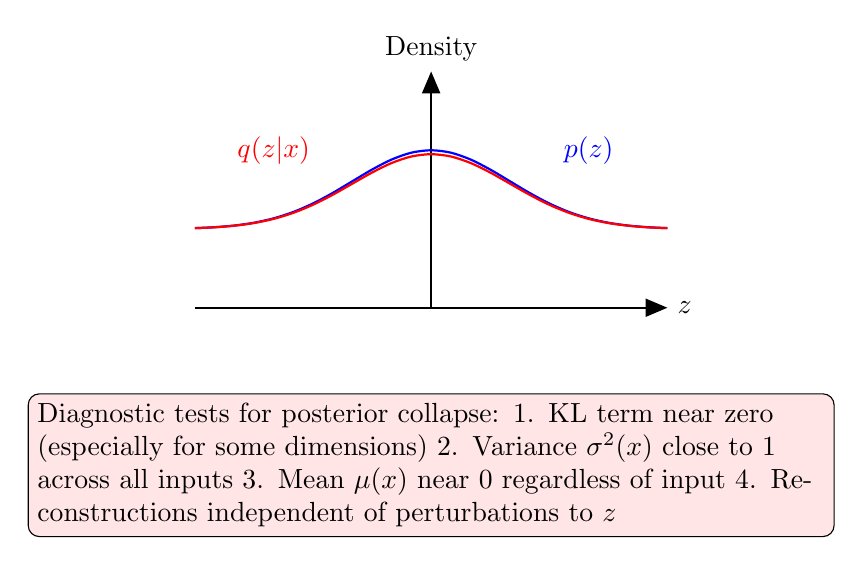
\begin{tikzpicture}
% Posterior collapse visualization
\draw[->,thick] (-3,0) -- (3,0) node[right] {$z$};
\draw[->,thick] (0,0) -- (0,3) node[above] {Density};

% Prior
\draw[domain=-3:3, smooth, variable=\x, blue, thick] 
  plot ({\x}, {1+exp(-\x*\x/2)});
\node[blue] at (2,2) {$p(z)$};

% Collapsed posterior
\draw[domain=-3:3, smooth, variable=\x, red, thick] 
  plot ({\x}, {1+exp(-\x*\x/2)*0.95});
\node[red] at (-2,2) {$q(z|x)$};

% Diagnostic
\node[rectangle,draw,fill=red!10,rounded corners,text width=10cm] at (0,-2) {
Diagnostic tests for posterior collapse:
1. KL term near zero (especially for some dimensions)
2. Variance $\sigma^2(x)$ close to 1 across all inputs
3. Mean $\mu(x)$ near 0 regardless of input
4. Reconstructions independent of perturbations to $z$
};
\end{tikzpicture}
\end{center}
\end{frame}


\begin{frame}{KL Warm-up Schedules}
\begin{itemize}
\item Strategy: Gradually increase weight of KL term during training
\item Implementation:
\begin{align}
\mathcal{L}(\theta, \phi; x, \beta_t) = \mathbb{E}_{q(z|x)}[\log p(x|z)] - \beta_t \cdot D_{KL}(q(z|x) \| p(z))
\end{align}
where $\beta_t$ increases from 0 to final value over training
\item Benefits:
  \begin{itemize}
  \item Helps avoid posterior collapse
  \item Allows encoder/decoder to initialize effectively
  \item Focuses on reconstruction first, then regularization
  \end{itemize}
\end{itemize}

\end{frame}

\begin{frame}


\begin{center}
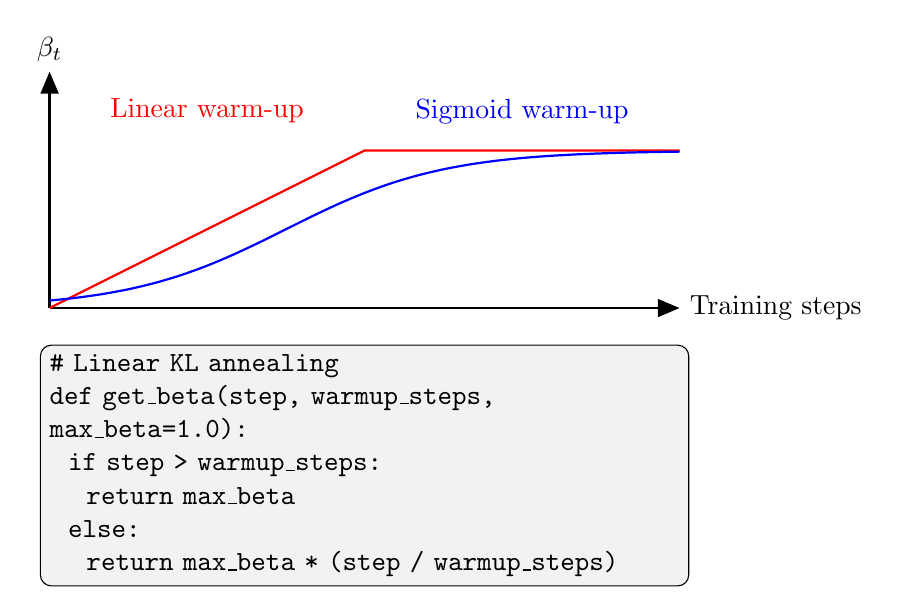
\begin{tikzpicture}
% Warm-up schedules
\draw[->,thick] (0,0) -- (8,0) node[right] {Training steps};
\draw[->,thick] (0,0) -- (0,3) node[above] {$\beta_t$};

% Linear schedule
\draw[red,thick] (0,0) -- (4,2) -- (8,2);
\node[red] at (2,2.5) {Linear warm-up};

% Sigmoid schedule
\draw[domain=0:8, smooth, variable=\x, blue, thick]
  plot ({\x}, {2/(1+exp(-(\x-3)))});
\node[blue] at (6,2.5) {Sigmoid warm-up};

% Implementation
\node[rectangle,draw,fill=gray!10,rounded corners,text width=8cm] at (4,-2) {
\texttt{\# Linear KL annealing}\\
\texttt{def get\_beta(step, warmup\_steps, max\_beta=1.0):}\\
\texttt{~~if step > warmup\_steps:}\\
\texttt{~~~~return max\_beta}\\
\texttt{~~else:}\\
\texttt{~~~~return max\_beta * (step / warmup\_steps)}
};
\end{tikzpicture}
\end{center}  
\end{frame}


\begin{frame}{Monitoring Training}
\begin{itemize}
\item Track multiple metrics during training:
  \begin{itemize}
  \item Total ELBO loss
  \item Reconstruction loss separately
  \item KL divergence separately
  \item Per-dimension KL 
  \item Sample quality metrics
  \end{itemize}
\item Visualization strategies:
  \begin{itemize}
  \item Original vs. reconstructed images
  \item Random samples from prior
  \item Latent space visualizations (t-SNE, PCA)
  \item Interpolations between samples
  \end{itemize}
\end{itemize}

\end{frame}


\begin{frame}
\begin{center}
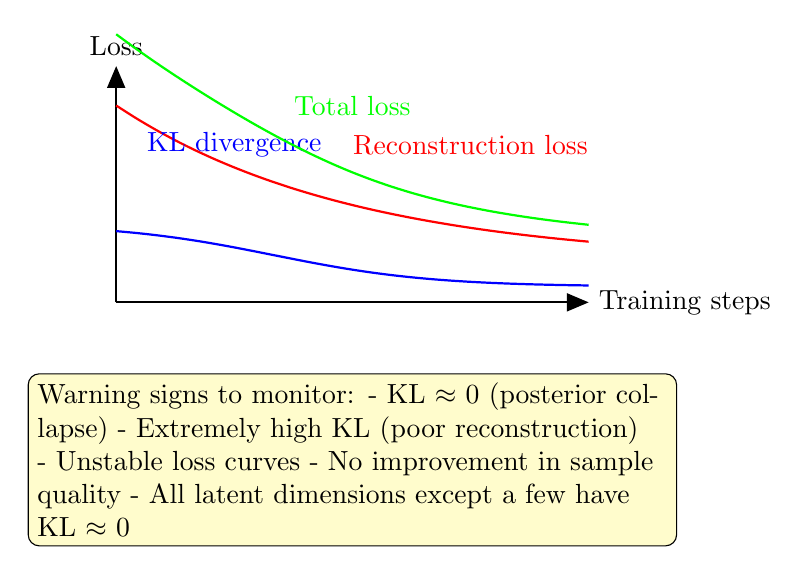
\begin{tikzpicture}
% Training curves
\draw[->,thick] (0,0) -- (6,0) node[right] {Training steps};
\draw[->,thick] (0,0) -- (0,3) node[above] {Loss};

% Loss curves
\draw[domain=0:6, smooth, variable=\x, red, thick]
  plot ({\x}, {2*exp(-\x/3) + 0.5});
\node[red] at (4.5,2) {Reconstruction loss};

\draw[domain=0:6, smooth, variable=\x, blue, thick]
  plot ({\x}, {0.2 + 0.8/(1+exp((\x-2)))});
\node[blue] at (1.5,2) {KL divergence};

\draw[domain=0:6, smooth, variable=\x, green, thick]
  plot ({\x}, {2*exp(-\x/3) + 0.5 + 0.2 + 0.8/(1+exp((\x-2)))});
\node[green] at (3,2.5) {Total loss};

% Warning signs
\node[rectangle,draw,fill=yellow!20,rounded corners,text width=8cm] at (3,-2) {
Warning signs to monitor:
- KL $\approx$ 0 (posterior collapse)
- Extremely high KL (poor reconstruction)
- Unstable loss curves
- No improvement in sample quality
- All latent dimensions except a few have KL $\approx$ 0
};
\end{tikzpicture}
\end{center}
    
\end{frame}



%%%%%%%%%%%%%%%%%%%%%%%%%%%%%%%%%%%%%%%%%%%%%%%%%%%%%%%%%%%%%%%%%%%%%%%
% Section 3.4: Conditional VAEs (20 minutes)
%%%%%%%%%%%%%%%%%%%%%%%%%%%%%%%%%%%%%%%%%%%%%%%%%%%%%%%%%%%%%%%%%%%%%%%
\section{Conditional VAEs}


\begin{frame}{Conditional VAEs}
\begin{itemize}
\item Motivation for conditional generation
\item Extending VAEs with auxiliary information
\item Graphical model formulation
\item Conditional ELBO objective
\item Conditioning mechanisms
\item Implementation examples
\item Applications and use cases
\item Best practices and pitfalls
\end{itemize}

\begin{center}
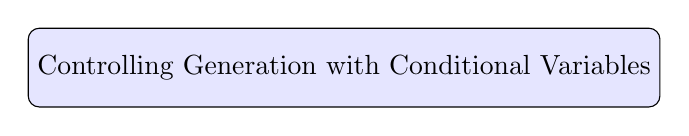
\begin{tikzpicture}
\node[rectangle,draw,fill=blue!10,rounded corners,minimum width=8cm,minimum height=1cm] at (0,0) {Controlling Generation with Conditional Variables};
\end{tikzpicture}
\end{center}
\end{frame}


\begin{frame}{Conditioning on Auxiliary Information $c$}
\begin{itemize}
\item Conditioning variable $c$ can be:
  \begin{itemize}
  \item Discrete: Class labels, categorical attributes
  \item Continuous: Real-valued properties
  \item Structured: Text, graphs, other objects
  \end{itemize}
\item Encoding methods for $c$:
  \begin{itemize}
  \item One-hot encoding for discrete variables
  \item Normalized values for continuous properties
  \item Embeddings for complex structures
  \end{itemize}
\item $c$ is provided during both training and generation
\end{itemize}

\begin{center}
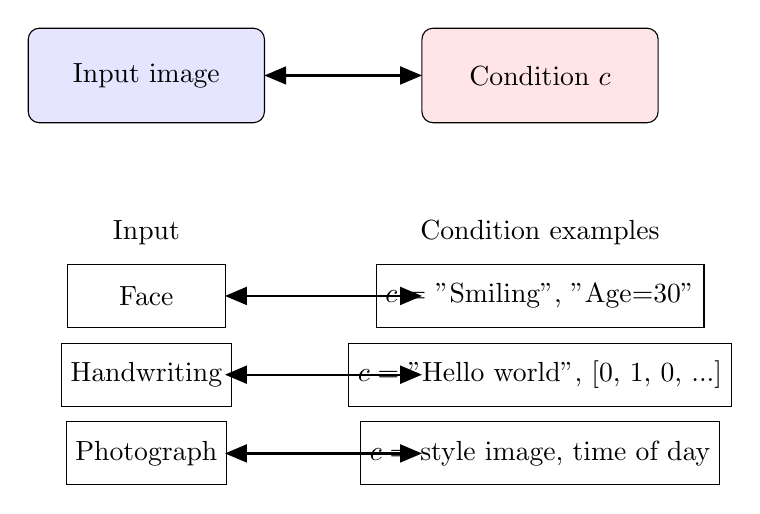
\begin{tikzpicture}
% Conditioning examples
\node[rectangle,draw,fill=blue!10,rounded corners,minimum width=3cm, minimum height=1.2cm] (image) at (0,0) {Input image};
\node[rectangle,draw,fill=red!10,rounded corners,minimum width=3cm, minimum height=1.2cm] (attr) at (5,0) {Condition $c$};

% Different types
\node at (0,-2) {Input};
\node at (5,-2) {Condition examples};

\node[rectangle,draw,minimum width=2cm, minimum height=0.8cm] at (0,-2.8) {Face};
\node[rectangle,draw,minimum width=2cm, minimum height=0.8cm] at (5,-2.8) {$c = $ "Smiling", "Age=30"};

\node[rectangle,draw,minimum width=2cm, minimum height=0.8cm] at (0,-3.8) {Handwriting};
\node[rectangle,draw,minimum width=2cm, minimum height=0.8cm] at (5,-3.8) {$c = $ "Hello world", [0, 1, 0, ...]};

\node[rectangle,draw,minimum width=2cm, minimum height=0.8cm] at (0,-4.8) {Photograph};
\node[rectangle,draw,minimum width=2cm, minimum height=0.8cm] at (5,-4.8) {$c = $ style image, time of day};

\draw[<->,thick] (1.5,0) -- (3.5,0);
\draw[<->,thick] (1,-2.8) -- (3.5,-2.8);
\draw[<->,thick] (1,-3.8) -- (3.5,-3.8);
\draw[<->,thick] (1,-4.8) -- (3.5,-4.8);
\end{tikzpicture}
\end{center}
\end{frame}


\begin{frame}{Graphical Model Formulation}
\begin{itemize}
\item Standard VAE:
  \begin{itemize}
  \item Prior: $p(z)$
  \item Likelihood: $p(x|z)$
  \item Approximate posterior: $q(z|x)$
  \end{itemize}
\item Conditional VAE:
  \begin{itemize}
  \item Conditional prior: $p(z|c)$
  \item Conditional likelihood: $p(x|z,c)$
  \item Conditional approximate posterior: $q(z|x,c)$
  \end{itemize}
\item Goal: model $p(x|c)$ instead of $p(x)$
\end{itemize}


\end{frame}


\begin{frame}

\begin{center}
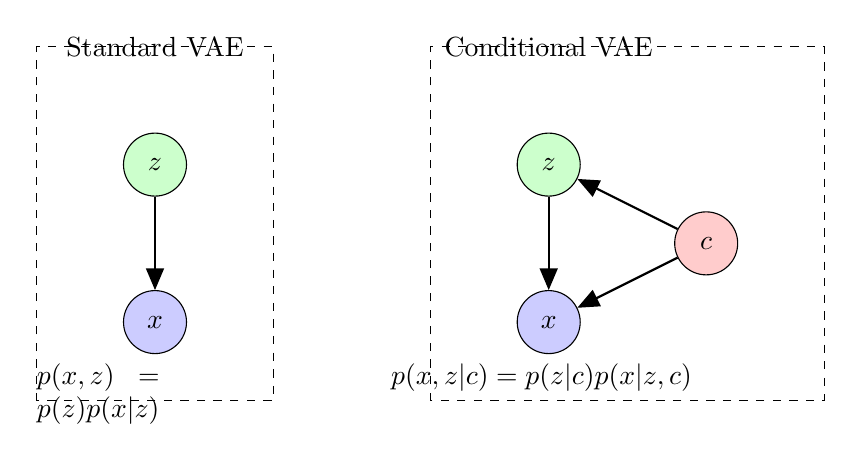
\begin{tikzpicture}
% Standard VAE graphical model
\node at (-3,1.5) {Standard VAE};
\node[circle,draw,fill=green!20,minimum size=0.8cm] (z1) at (-3,0) {$z$};
\node[circle,draw,fill=blue!20,minimum size=0.8cm] (x1) at (-3,-2) {$x$};
\draw[->,thick] (z1) -- (x1);
\node[below,text width=3cm] at (x1.south) {$p(x,z) = p(z)p(x|z)$};

% cVAE graphical model
\node at (2,1.5) {Conditional VAE};
\node[circle,draw,fill=green!20,minimum size=0.8cm] (z2) at (2,0) {$z$};
\node[circle,draw,fill=blue!20,minimum size=0.8cm] (x2) at (2,-2) {$x$};
\node[circle,draw,fill=red!20,minimum size=0.8cm] (c2) at (4,-1) {$c$};
\draw[->,thick] (z2) -- (x2);
\draw[->,thick] (c2) -- (x2);
\draw[->,thick] (c2) -- (z2);
\node[below,text width=4cm] at (x2.south) {$p(x,z|c) = p(z|c)p(x|z,c)$};

% Plate notation for training
\draw[dashed] (-4.5,-3) rectangle (-1.5,1.5);
\draw[dashed] (0.5,-3) rectangle (5.5,1.5);
\end{tikzpicture}
\end{center}
    
\end{frame}

\begin{frame}{Encoder: $q(z|x,c)$}
\begin{itemize}
\item Conditional encoder approximates $p(z|x,c)$
\item Inputs: data $x$ and condition $c$
\item Outputs: parameters of $q(z|x,c) = \mathcal{N}(z; \mu(x,c), \sigma^2(x,c))$
\item Implementation options:
  \begin{itemize}
  \item Concatenate $c$ to input $x$
  \item \textbf{Process $c$ separately and merge features}
  \end{itemize}
\end{itemize}

\begin{center}
    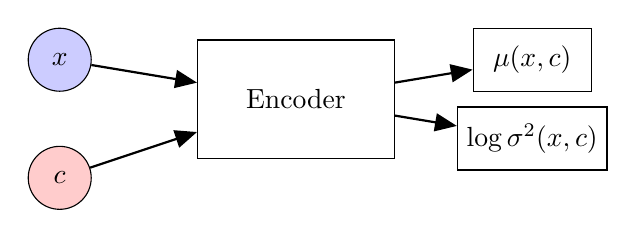
\begin{tikzpicture}
        % Conditional encoder
\node[circle,draw,fill=blue!20,minimum size=0.8cm] (x) at (0,0) {$x$};
\node[circle,draw,fill=red!20,minimum size=0.8cm] (c) at (0,-1.5) {$c$};
\node[rectangle,draw,minimum width=2.5cm,minimum height=1.5cm] (enc) at (3,-0.5) {Encoder};
\node[rectangle,draw,minimum width=1.5cm,minimum height=0.8cm] (mu) at (6,0) {$\mu(x,c)$};
\node[rectangle,draw,minimum width=1.5cm,minimum height=0.8cm] (logvar) at (6,-1) {$\log\sigma^2(x,c)$};

\draw[->,thick] (x) -- (enc);
\draw[->,thick] (c) -- (enc);
\draw[->,thick] (enc) -- (mu);
\draw[->,thick] (enc) -- (logvar);
    \end{tikzpicture}
\end{center}
\end{frame}


\begin{frame}
\centering
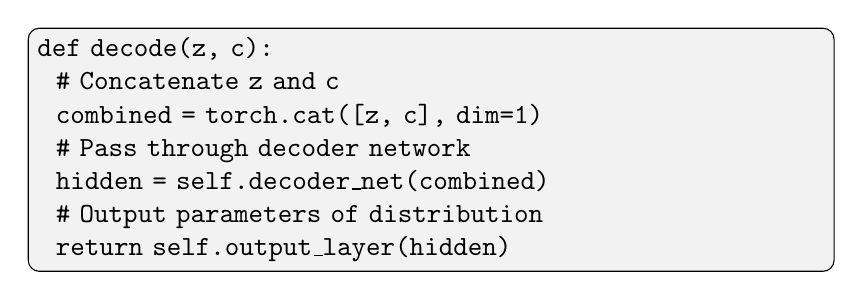
\begin{tikzpicture}
    % Example implementation
\node[rectangle,draw,fill=gray!10,rounded corners,text width=10cm] at (3,-3) {
\texttt{def decode(z, c):}\\
\texttt{~~\# Concatenate z and c}\\
\texttt{~~combined = torch.cat([z, c], dim=1)}\\
\texttt{~~\# Pass through decoder network}\\
\texttt{~~hidden = self.decoder\_net(combined)}\\
\texttt{~~\# Output parameters of distribution}\\
\texttt{~~return self.output\_layer(hidden)}
};
\end{tikzpicture}
\end{frame}

\begin{frame}{Decoder: $p(x|z,c)$}
\begin{itemize}
\item Conditional decoder models $p(x|z,c)$
\item Inputs: latent code $z$ and condition $c$
\item Outputs: parameters of data distribution
\item Design parallels conditional encoder:
  \begin{itemize}
  \item Concatenate $c$ to latent code $z$
  \item Process $c$ separately and combine with $z$
  \end{itemize}
\end{itemize}

\begin{center}
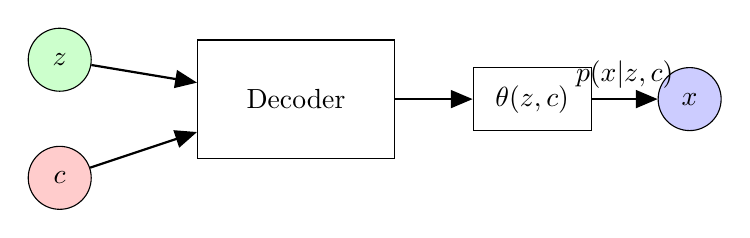
\begin{tikzpicture}
% Conditional decoder
\node[circle,draw,fill=green!20,minimum size=0.8cm] (z) at (0,0) {$z$};
\node[circle,draw,fill=red!20,minimum size=0.8cm] (c) at (0,-1.5) {$c$};
\node[rectangle,draw,minimum width=2.5cm,minimum height=1.5cm] (dec) at (3,-0.5) {Decoder};
\node[rectangle,draw,minimum width=1.5cm,minimum height=0.8cm] (out) at (6,-0.5) {$\theta(z,c)$};
\node[circle,draw,fill=blue!20,minimum size=0.8cm] (x) at (8,-0.5) {$x$};

\draw[->,thick] (z) -- (dec);
\draw[->,thick] (c) -- (dec);
\draw[->,thick] (dec) -- (out);
\draw[->,thick] (out) -- (x) node[midway,above] {$p(x|z,c)$};


\end{tikzpicture}
\end{center}
\end{frame}






\begin{frame}

\begin{center}
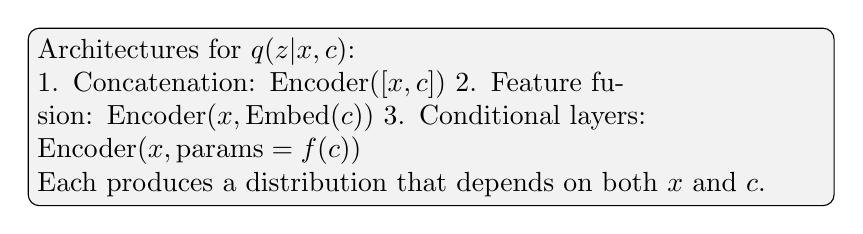
\begin{tikzpicture}


% Architectures
\node[rectangle,draw,fill=gray!10,rounded corners,text width=10cm] at (3,-3) {
Architectures for $q(z|x,c)$:

1. Concatenation: $\text{Encoder}([x, c])$
2. Feature fusion: $\text{Encoder}(x, \text{Embed}(c))$
3. Conditional layers: $\text{Encoder}(x, \text{params}=f(c))$

Each produces a distribution that depends on both $x$ and $c$.
};
\end{tikzpicture}
\end{center}
    
\end{frame}



\begin{frame}{Conditional ELBO}
\textbf{Goal:} Maximize conditional log-likelihood $\log p(x|c)$

\textbf{Derivation} parallels standard ELBO:
\[
\log p(x|c) \geq \mathbb{E}_{q(z|x,c)}[\log p(x|z,c)] - D_{KL}(q(z|x,c) \| p(z|c))
\]

\textbf{Components:}

Conditional reconstruction: $\mathbb{E}_{q(z|x,c)}[\log p(x|z,c)]$

Conditional KL divergence: $D_{KL}(q(z|x,c) \| p(z|c))$

\begin{center}
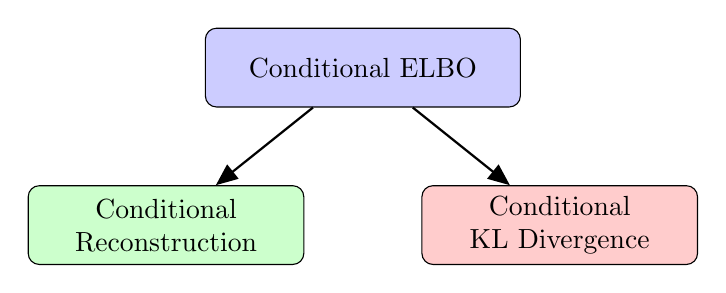
\begin{tikzpicture}
% ELBO components
\node[rectangle,draw,fill=blue!20,rounded corners,minimum width=4cm,minimum height=1cm] (elbo) at (0,0) {Conditional ELBO};
\node[rectangle,draw,fill=green!20,rounded corners,minimum width=3.5cm,minimum height=1cm,align=center] (rec) at (-2.5,-2) {Conditional\\Reconstruction};
\node[rectangle,draw,fill=red!20,rounded corners,minimum width=3.5cm,minimum height=1cm,align=center] (kl) at (2.5,-2) {Conditional\\KL Divergence};

\draw[->,thick] (elbo) -- (rec);
\draw[->,thick] (elbo) -- (kl);


\end{tikzpicture}
\end{center}
\end{frame}
\begin{frame}{Hands-On Session: VAE}
\centering
\textbf{Variational Autoencoder (VAE)}
\begin{figure}
    \centering
    
\includegraphics[width=0.3\linewidth]{images/vae_hands_on_qr.png}
\end{figure}
\begin{itemize}
    \item \small Click here to download/open the notebook: \attachfile[color=0.5 0.5 0.5]{hands-on/VAE_hands_on.ipynb} (or click \href{run:hands-on/VAE_hands_on.ipynb}{here} to open if supported)
    \item \footnotesize Public Repository: \url{https://github.com/mariganeshkumar/tce_gen_ai_slide_deck_2/blob/main/hands-on/VAE_hands_on.ipynb}
\end{itemize}
\end{frame}

\begin{frame}{Hands-On Session: CVAE}
\centering
\textbf{Conditional Variational Autoencoder (CVAE)}
\begin{figure}
    \centering
    
\includegraphics[width=0.3\linewidth]{images/cvae_hands_on_qr.png}
\end{figure}
\begin{itemize}
    \item \small Click here to download/open the notebook: \attachfile[color=0.5 0.5 0.5]{hands-on/CVAE_hands_on.ipynb} (or click \href{run:hands-on/CVAE_hands_on.ipynb}{here} to open if supported)
    \item \footnotesize Public Repository: \url{https://github.com/mariganeshkumar/tce_gen_ai_slide_deck_2/blob/main/hands-on/CVAE_hands_on.ipynb}
\end{itemize}
\end{frame}

\begin{frame}{Summary: Recall the Journey}
  \begin{itemize}
    \item \textbf{The Baseline}: Standard Autoencoders map inputs to \textbf{deterministic points}. Good for compression, bad for generation.
    \item \textbf{The Upgrade}: VAEs map inputs to \textbf{probability distributions} ($\mu, \sigma$) for a continuous latent space.
    \item \textbf{The Hurdle}: How to backpropagate through a random sampling node?
    \item \textbf{The Fix}: The \textbf{Reparameterization Trick} ($\mu + \sigma \cdot \epsilon$) isolates the randomness!
    \item \textbf{The Goal}: \textbf{ELBO} balances reconstruction quality with latent space smoothness (KL divergence).
    \item \textbf{The Extension}: \textbf{CVAEs} allow controlled generation by feeding a condition $c$.
  \end{itemize}
\end{frame}

\end{document}
